%\pagenumbering{arabic}\setcounter{page}{1}
\chapter{Distributions of Random Variables}
\label{chapterDistributionsofRandomVariables}
%%start relabeling as 2.1 etc
%\pagestyle{myheadings}  \markboth{\ref{sec.matrix}.
%\titleref{sec.matrix}}{}
\setcounter{equation}{0}


\section{Distributions of Discrete Random Variables}

\subsection{Bernoulli Distribution}
\label{sectionBernouli}
\index{Distribution!Bernoulli}

A \textit{Bernoulli} random variable is a discrete random variable that has exactly two possible outcomes: \textit{success} or \textit{failure}. 
The terms \textit{success} and \textit{failure} are relative to the problem being analyzed. 
For example, in a problem regarding quality control we may consider obtaining a faulty part as a success (while in real life this is typically not regarded as being a good thing).\\

The mass function of a Bernoulli random variable is given in mass function $\ref{pmfBernoulli}$ below. 
If $X$ is a Bernoulli random variable then $X$ takes the value of 1 with probability of success $p$ and the value of 0 with probability $1-p$.

\begin{pmf}[The Bernoulli Distribution]
\label{pmfBernoulli}
Let $X \sim \text{Bernoulli}(p)$. 
The mass function of $X$ is
	\begin{align}
	P(X = x) & = p^{x}(1-p)^{1-x}, \quad x = 0, 1
	\end{align}
where $p$ represents the probability of success.
\end{pmf}

\noindent
Another way to represent the Bernoulli Distribution is
\begin{align}
P(X=x)	&=
	\begin{cases}
	p        & \text{if } x = 1 \\[0.5em]
	1-p        & \text{if } x = 0 \\
  \end{cases}
\end{align}

\noindent
This distribution can also be expressed in tabular form
\begin{center}
\def\arraystretch{1.5}
\begin{tabular}{c | c | c}
$X=x$	&	1	&	0	\\
\hline
$P(X=x)$	&	$p$	&	$1-p$	\\
\end{tabular}
\end{center}

\noindent
The simplest example of a Bernoulli random variable is the outcome of tossing a fair coin once. If we consider a success to be getting tails and a failure to be getting heads, the probability of a success is $p=0.5$ and the probability of a failure
is $1-p = 1-0.5 = 0.5$.

\begin{definition}[Mean and Variance of a Bernoulli Random Variable]
Let $X \sim \text{Bernoulli}~(p)$. 
The mean of $X$ is
	\begin{align}
	E(X) = \mu = p	\label{meanBernoulli}
	\end{align}
and the variance of $X$ is
	\begin{align}
	Var(X) = \sigma^{2} = p~(1-p)
	\end{align}
\end{definition}



\subsection{Binomial Distribution}
\index{Distribution!Binomial}

The \textit{binomial} distribution generalizes the Bernoulli distribution from a single trial to many trials.
We use this distribution when we $n$ independent Bernoulli trials occur and we are 
interested in $x$ successes occurring in those $n$ trials. 
The probability of success is denoted as $p$ and it is the same each of the $n$ trials. 
If $X$ is a binomial random variable it is denoted as $X \sim \text{Bin}(n, p)$ where $n$ is the number of trials and $p$ is the probability of a success on any trial.
The mass function of a binomial random variables involves the binomial coefficient
from definition $\ref{definitionBinomialCoefficient}$.

\begin{pmf}[Binomial  Distribution]
\label{pmfBinomial}
Let $X \sim \text{Bin}(n, p)$.
The probability of observing $x$ successes in these $n$ independent trials is given by
	\justifying
	\begin{equation}
	P(X = x) = {n \choose x} p^{x} (1 - p)^{n - x}
	\end{equation}
where
\begin{itemize}
\item[] $n$ represents the number of trials,
\item[] $x$ represents the number of successes,
\item[] $p$ represents the probability of success on any given trial,
\item[] $\displaystyle {n \choose x} = \frac{n!}{x!(n-x)!}$ is the binomial coefficient.
\end{itemize}
\end{pmf}

Let's examine mass function $\ref{pmfBinomial}$ closely. 
We have a total of $n$ trials in which we are interested in $x$ successes. 
As the $n$ trials have only two possible outcomes, if $x$ of these trials are successes 
then the remaining $n-x$ trials must be failures. 
Each success occurs with probability $p$ and each failure occurs with probability $1-p$.
The expression $p^{x} (1 - p)^{n - x}$ is the probability of obtaining $x$ successes and $n-x$ failures. 
The binomial coefficient ${n \choose x}$ accounts for all possible combinations of $x$ successes and $n-x$ failures in $n$ trials.\\

A simple example of a binomial random variable is tossing a coin 10 times and calculating the probability of obtaining 6 heads on any of these trials.

\begin{definition}[Mean and Variance of a Binomial Random Variable]
Let $X \sim Bin(n,p)$.
The mean of $X$ is
	\begin{align}
	E(X) = \mu = np
	\end{align}
and the variance of $X$ is
	\begin{align}
	Var(X) = \sigma^{2} = np~(1-p)
	\end{align}
\end{definition}


\begin{example}
Suppose $X \sim Bin(10,0.35)$. 
\begin{benumerate}
\item What is the mean of $X$?
\[ \mu = \mathbb{E}(X) = np = 10 \times 0.35 = 3.50 \]

\item What is the variance of $X$?
\[ \sigma^{2} = np(1-p) = 10 \times 0.35 (1-0.35) = 10 \times 0.2275 = 2.275 \]

\item What is the probability that $X=5$? 

The probability mass function of $X \sim Bin(10, 0.35)$ is
\[ P(X=x) = {10 \choose x}~(0.35)^{x}~(0.65)^{10-x} \]
Plugging in $x=5$,
\begin{align*}
P(X=5)	= {10 \choose 5}~(0.35)^{5}~0.65^{10-5} = 252 \times (0.35)^{5} \times (0.65)^{5} = 0.154
\end{align*}
 
\item What is the probability that $X \leq 5$?
\begin{align*}
P(X \leq 5) &= P(X=5) + P(X=4) + P(X=3) + P(X=2) + P(X=1) + P(X=0) \\
			&= \sum_{x=0}^{5} {10 \choose x}~0.35^{x} ~0.65^{10-x} \\
			&= {10 \choose 0}~0.35^{0}~0.65^{10} + {10 \choose 1}~0.35^{1}~0.65^{9} + {10 \choose 2}~0.35^{2}~0.65^{8} \\ &+ {10 \choose 3}~0.35^{3}~0.65^{7}+{10 \choose 4}~ 0.35^{4}~0.65^{6} + {10 \choose 5}~0.35^{5}~0.65^{5} \\
			&= 0.013 + 0.072 + 0.176 + 0.252 + 0.238 + 0.154 \\
			&= 0.905
\end{align*}

\item What is the probability that $X > 5$? 

$P(X>5)$ is the complement of $P(X \leq 5)$.
\begin{align*}
\Rightarrow P(X>5) = 1 - P(X \leq 5) = 1 - 0.905 = 0.095
\end{align*}

\item What is the probability that $X \geq 5$?

\[ P(X \geq 5) = P(X >5) + P(X=5) = 0.095 + 0.154 = 0.249 \]

\item What is the probability that $3 \leq X \leq 6$?

\[
P(3 \leq X \leq 6) 	= P(X=3) + P(X=4) + P(X=5) + P(X=6)
\]
From part (d), we know
\[P(X=5)=0.154,~~P(X=4)=0.238,~~P(X=3) = 0.252\]
We only need to find $P(X=6)$.
\begin{align*}
P(X = 6) &= {10 \choose 6}~0.35^6~0.65^4=0.069\\
\Rightarrow P(3 \leq X \leq 6) &= 0.252+0.238+0.154+0.069=0.713
\end{align*}
\end{benumerate}
\end{example}


\section{Distributions of Continuous Random Variables}

\subsection{Continuous Uniform Distribution}
\index{Distribution!Continuous uniform}

A \textit{continuous random variable} follows a \textit{uniform} probability distribution if any value within a defined interval is equally likely. If a random variable $X$ is distributed uniformly on interval $[a, b]$ we denote this as $X \sim \text{U}(a,b)$. The distribution function of a uniform random variable is very simple.

\hfill
\begin{pdf}[Continuous Uniform Distribution]
Let $X \sim \text{U}(a, b)$. The density function of $X$ is
	\[ f(x) = \left\{ 
		\begin{array}{l l}
		\displaystyle\frac{1}{(b - a)}	& \quad \text{for }  ~ a \leq x \leq b\\
		\hfill\\
		0 						& \quad \text{otherwise}
		\end{array} \right.\]
\end{pdf}

\begin{definition}[Mean and Variance of a Uniform Random Variable]
Let $X \sim \text{U}(a,b)$. The mean of $X$ is
	\begin{equation}
	\mathbb{E}(X) = \mu = \displaystyle\frac{a + b}{2}
	\end{equation}
and the variance of $X$ is
	\begin{equation}
	Var(X) = \sigma^2 = \displaystyle\frac{(b - a)^2}{12}
	\end{equation}
\end{definition}





\subsection{Normal Distribution}
\label{sectionNormalDistribution}
\index{Distribution!Normal}

The \textit{Normal} distribution (also referred to as the \textit{Gaussian} distribution) is an extremely important distribution in statistics and many other areas including mathematics, econometrics, finance, physics, astronomy etc. 
The normal distribution models many real life processes and events.
This distribution is the bell curve that we are used to seeing.
If $X$ is a random variable which follows a normal distribution we denote
this as $X \sim N(\mu, \sigma^{2})$ where $\mu$ and $\sigma^{2}$ are the
mean and standard deviation respectively

\begin{pdf}[Normal Distribution]
Let $X \sim \text{N}(\mu, \sigma^{2})$.
The density function of $X$ is
\begin{equation}
f(x) = \displaystyle\frac{1}{ ( \sqrt{2 \pi} ) \sigma } e^{ \displaystyle -\frac{ (x - \mu)^{2} }{ 2 \sigma^{2}}  }	~\quad~	-\infty < x < +\infty
\end{equation}
\end{pdf}

The normal distribution is completely described by the mean $\mu$ and standard deviation $\sigma$.
Note that the support of the normal distribution is the entire real number line 
(i.e. the support is infinite).


\begin{figure}[H]
\vspace*{-0.5cm}
\begin{center}
%\begin{picture}%(100,100)
%\put(0,57){ \includegraphics[width=6.5cm]{norm_0.pdf} } 
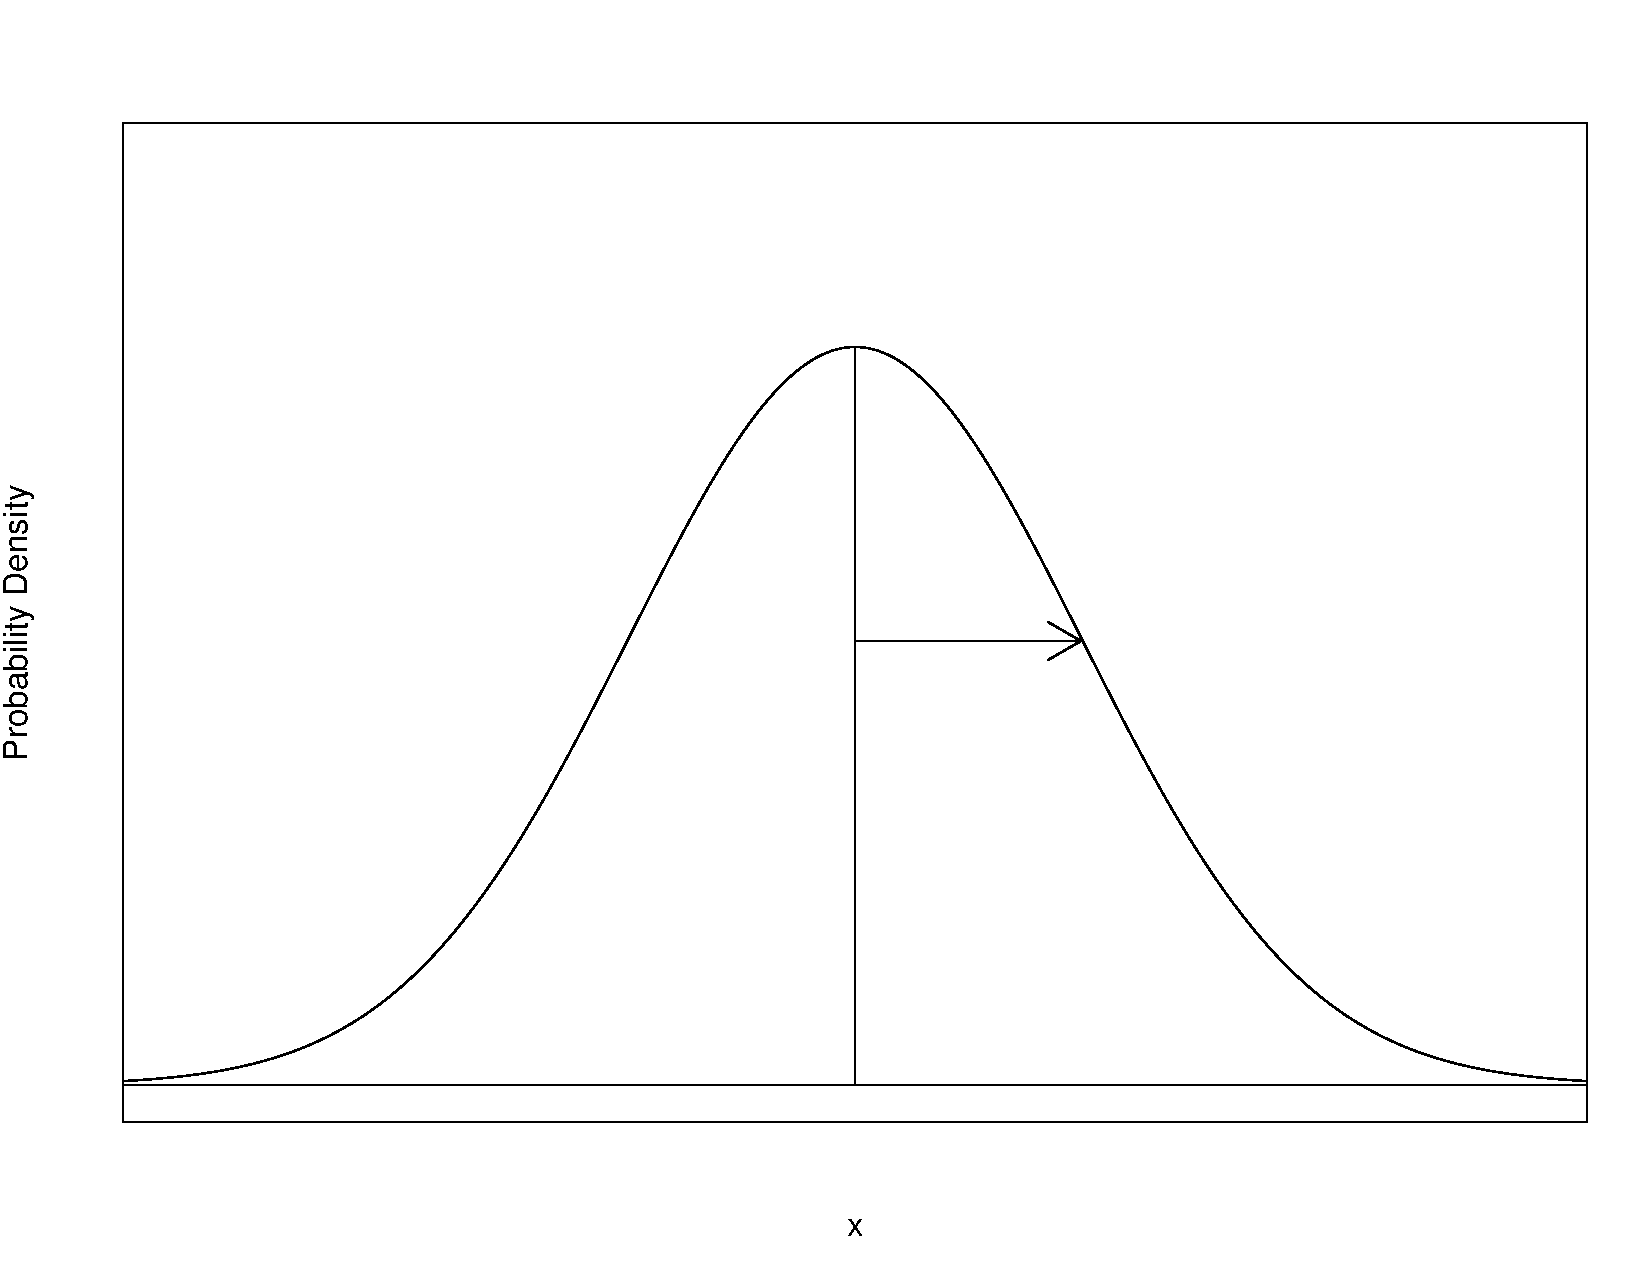
\includegraphics[scale=0.40]{Section4/norm0.pdf}
\put (-477, 31.0){\makebox[0.7\textwidth][r]{$\mu$ }}
\put (-460, 125.0){\makebox[0.7\textwidth][r]{$\sigma$ }}
%\end{picture}
\end{center}
\vspace{-1cm}
\caption{The normal distribution}
\end{figure}


%\pagebreak

%\vspace*{-0.5cm}
\noindent
The normal distribution is symmetric about $\mu$
(i.e. 0.5 probability below $\mu$ and 0.5 probability above $\mu$).
The mean, median and mode are all the same value of $\mu$.
Some examples of normal distributions with different means and standard deviations are given in 
Figure $\ref{figureNormalExamples}$.



\begin{figure}[H]
\label{figureNormalExamples}
\vspace*{-0.25cm}
\begin{center}
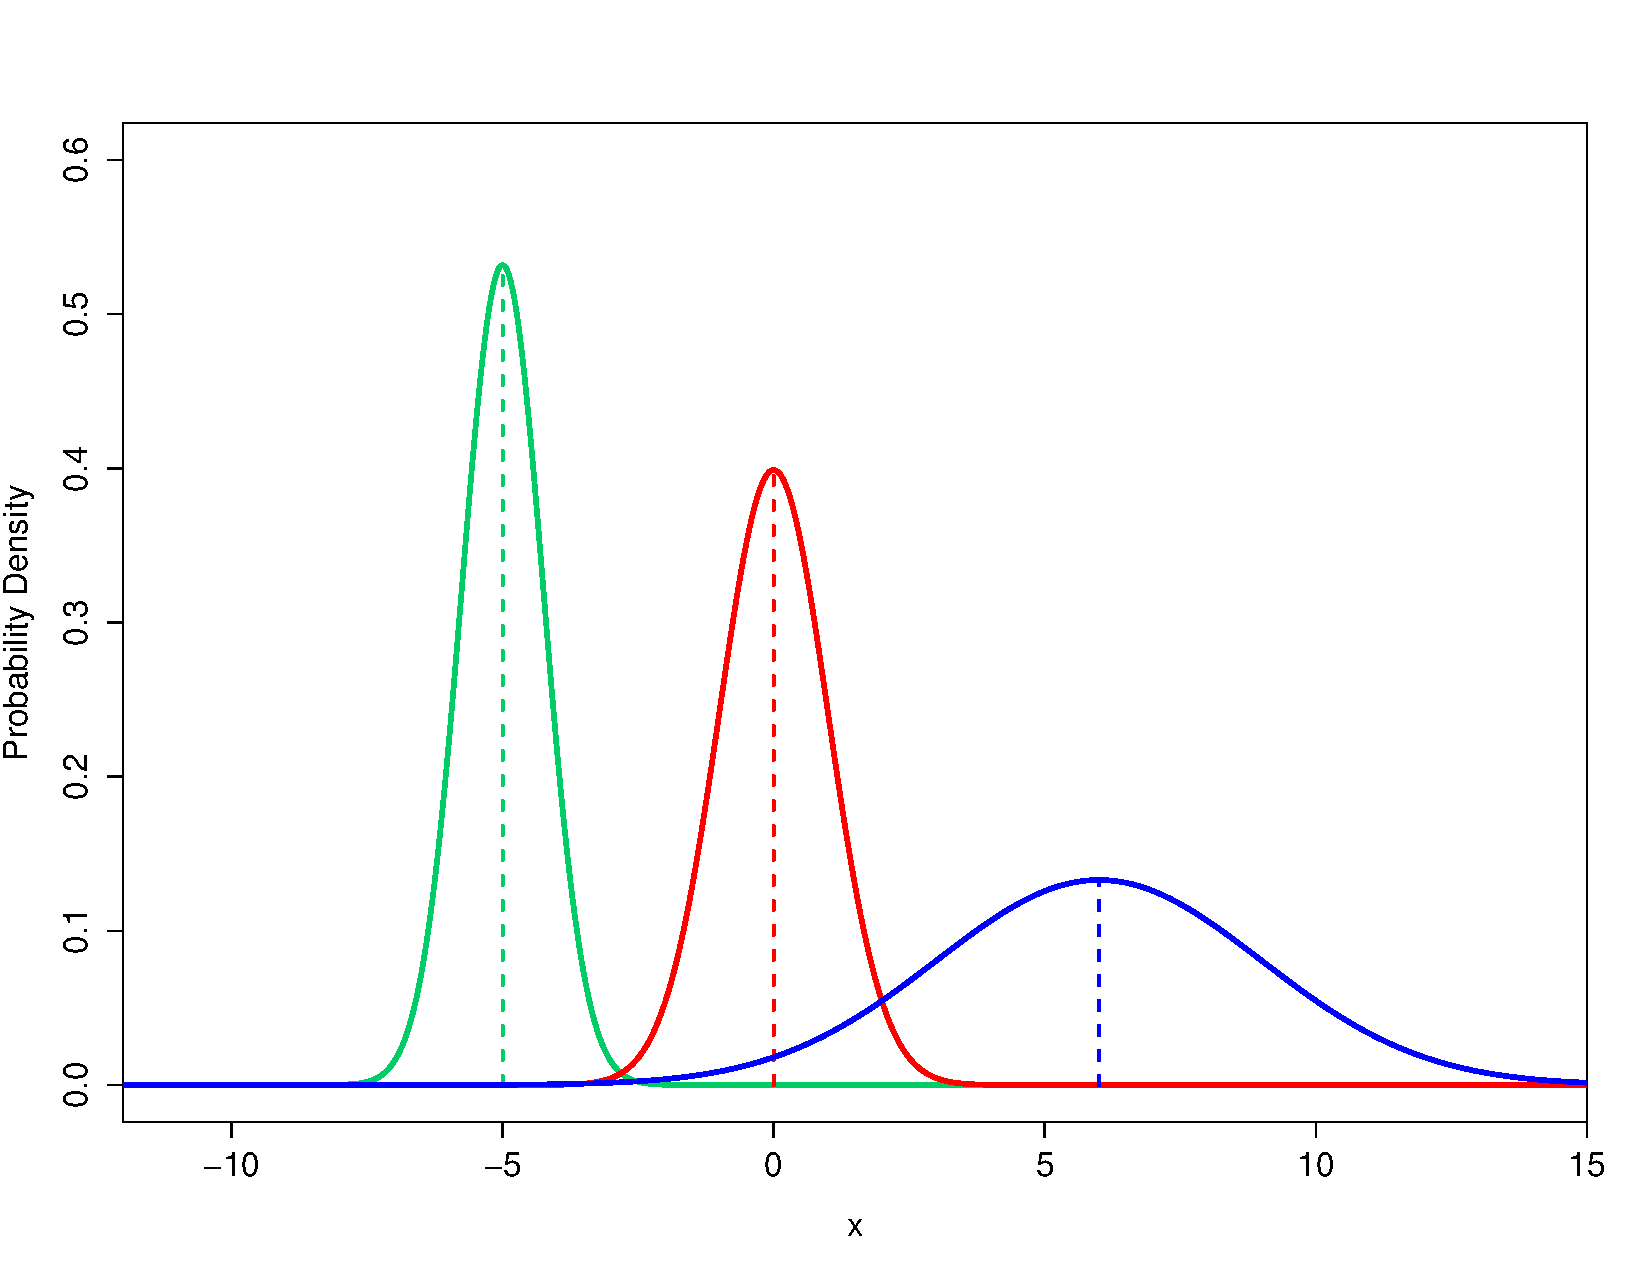
\includegraphics[scale=0.40]{Section4/normalexamples.pdf}
\tiny
\put (-520, 205.0){\makebox[0.7\textwidth][r]{ \textcolor[RGB]{0,205,102}{$\mu= -5,~ \sigma=0.75$} }}
\put (-475, 165.0){\makebox[0.7\textwidth][r]{ \textcolor{red}{$\mu= 0,~ \sigma= 1$} }}
\put (-410, 86.0){\makebox[0.7\textwidth][r]{ \textcolor{blue}{$\mu= 6,~ \sigma= 3$} }}
\vspace{-0.5cm}
\caption{Examples of normal distributions with different means and standard deviations}
\end{center}
\end{figure}






\subsubsection{The Standard Normal Distribution}

The \textit{standard normal} distribution is a normal distribution with $\mu = 0$ and $\sigma = 1$.

\begin{figure}[H]
\begin{center}
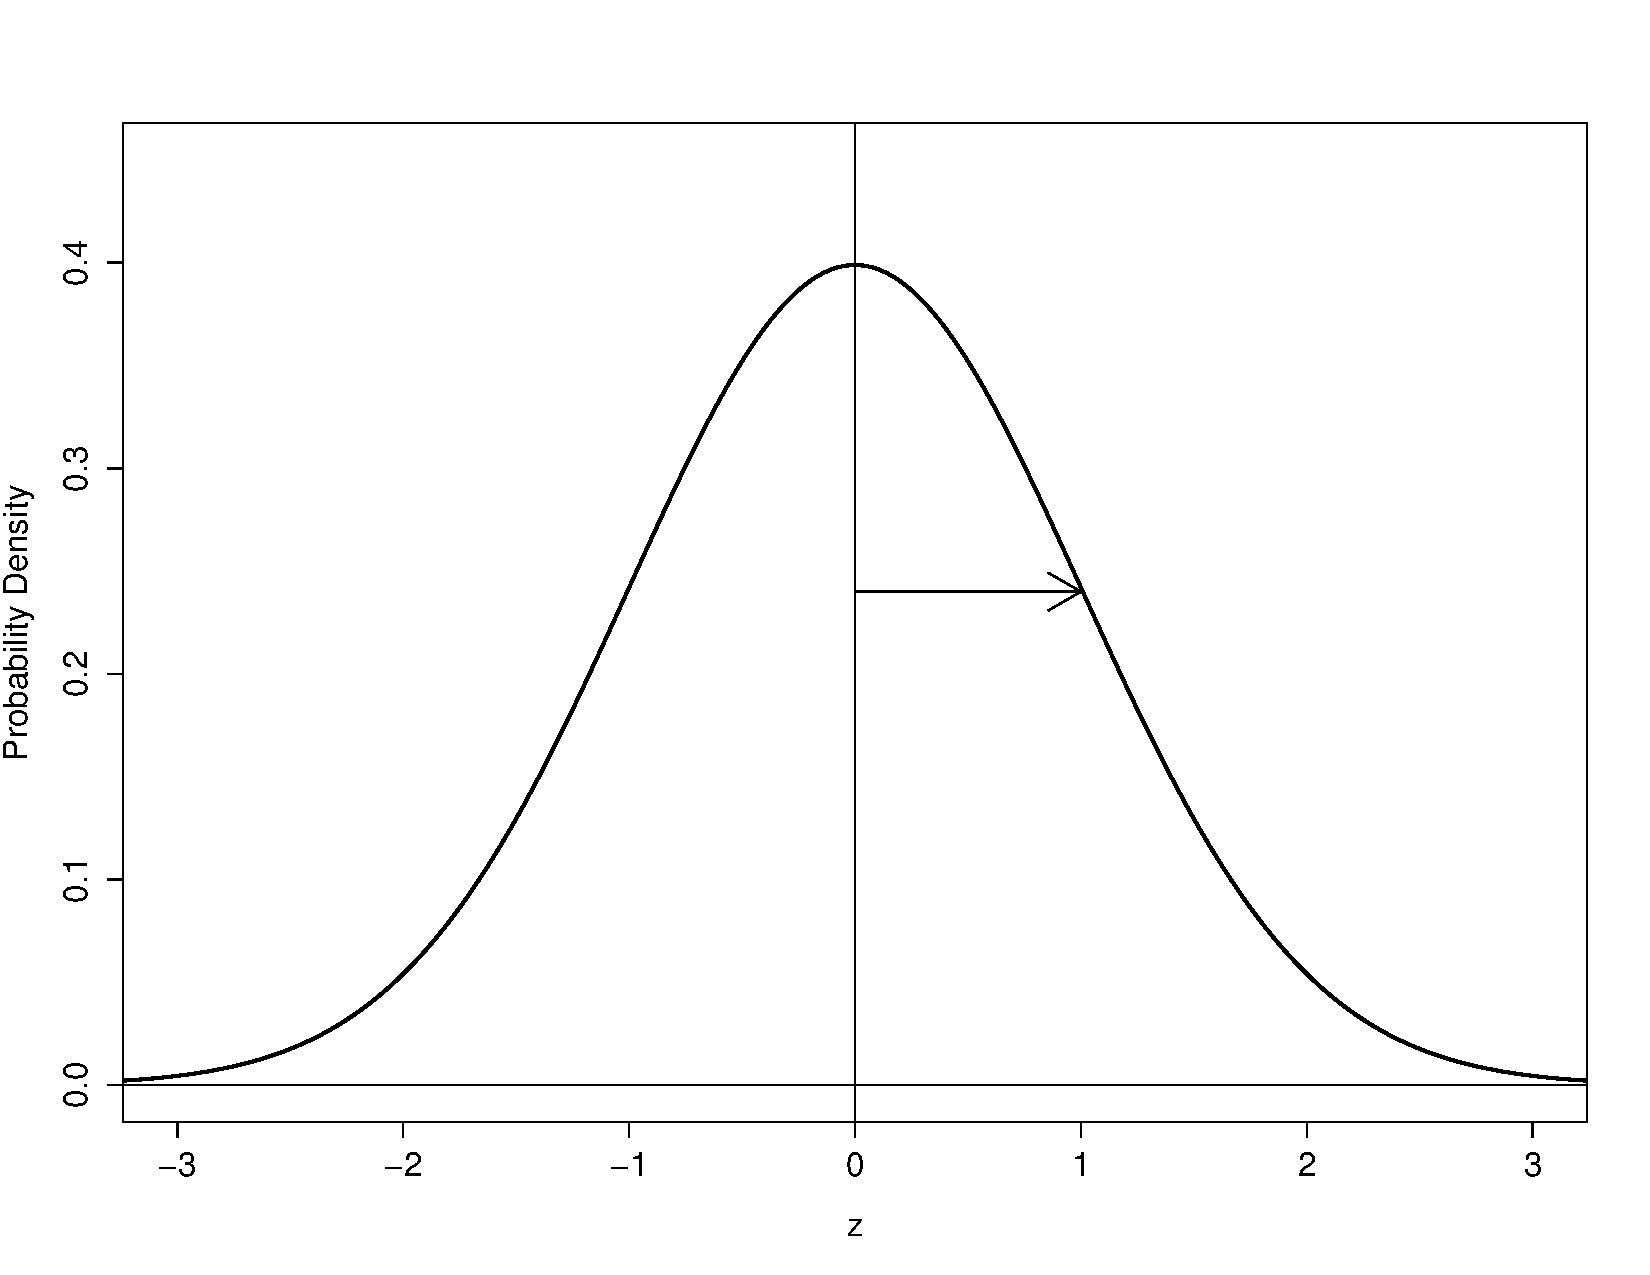
\includegraphics[scale=0.38]{Section4/z_table_0.pdf}
\small
\put (-477.5, 37.5){\makebox[0.7\textwidth][r]{$\mu = 0$ }}
\put (-445, 130){\makebox[0.7\textwidth][r]{$\sigma = 1$ }}
\vspace{-0.5cm}
\caption{The standard normal distribution.}
\end{center}
\end{figure}

A random variable that follows a standard normal distribution is usually associated with the letter $Z$ and is denoted as $Z \sim N(0, ~ 1)$. Probabilities under the standard normal curve are in a table at the back of this text {\textcolor{red}{(Appendix ???: Table ???. An equivalent copy of this table is also on courselink).} } It is extremely important to familiarize yourself with this table.\\

A normal distribution can have any mean and any standard deviation, so there are infinitely many of them. We transform a probability question about a random variable that follows any normal distribution in to an equivalent problem in terms of the 
standard normal distribution. This way we have a single standard tool (i.e. the standard normal table) which we can use to solve problems involving a normal distribution.

\begin{definition}[$Z$ score]	\index{Z score}
The $Z$ score of an observation is the number of standard deviations by which it falls above or below the mean.
\end{definition}

\begin{figure}[H]
\begin{center}
\begin{tabular}{ccc}
\normalsize\underline{Original Problem}	& \hspace{5.2cm}		
								& \normalsize\underline{Equivalent Problem}\\
\footnotesize (in terms of $x$)	&		& \footnotesize (in terms of $z$)
\end{tabular}
\end{center}

\begin{center}
*\hspace*{-10px}
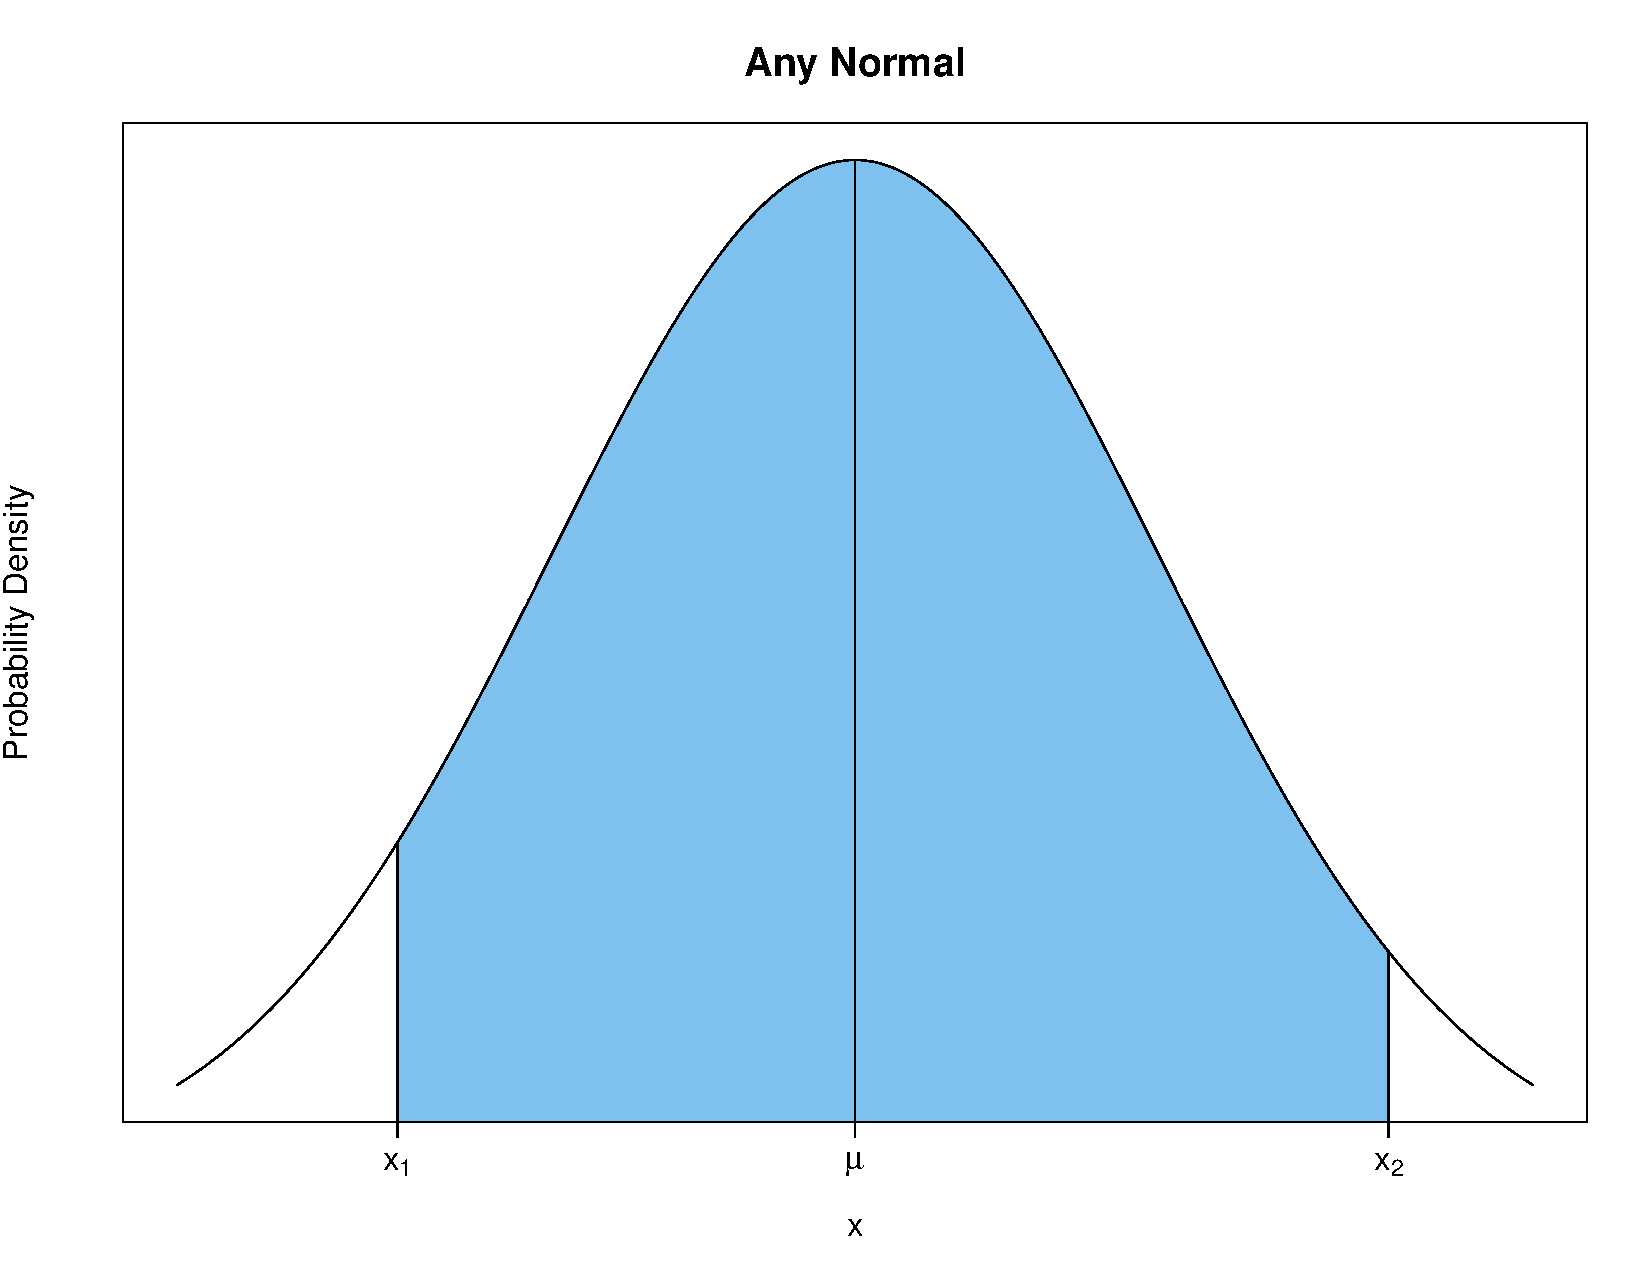
\includegraphics[width=7.250cm]{Section4/transform_any_normal.pdf} \hspace{1.75cm}
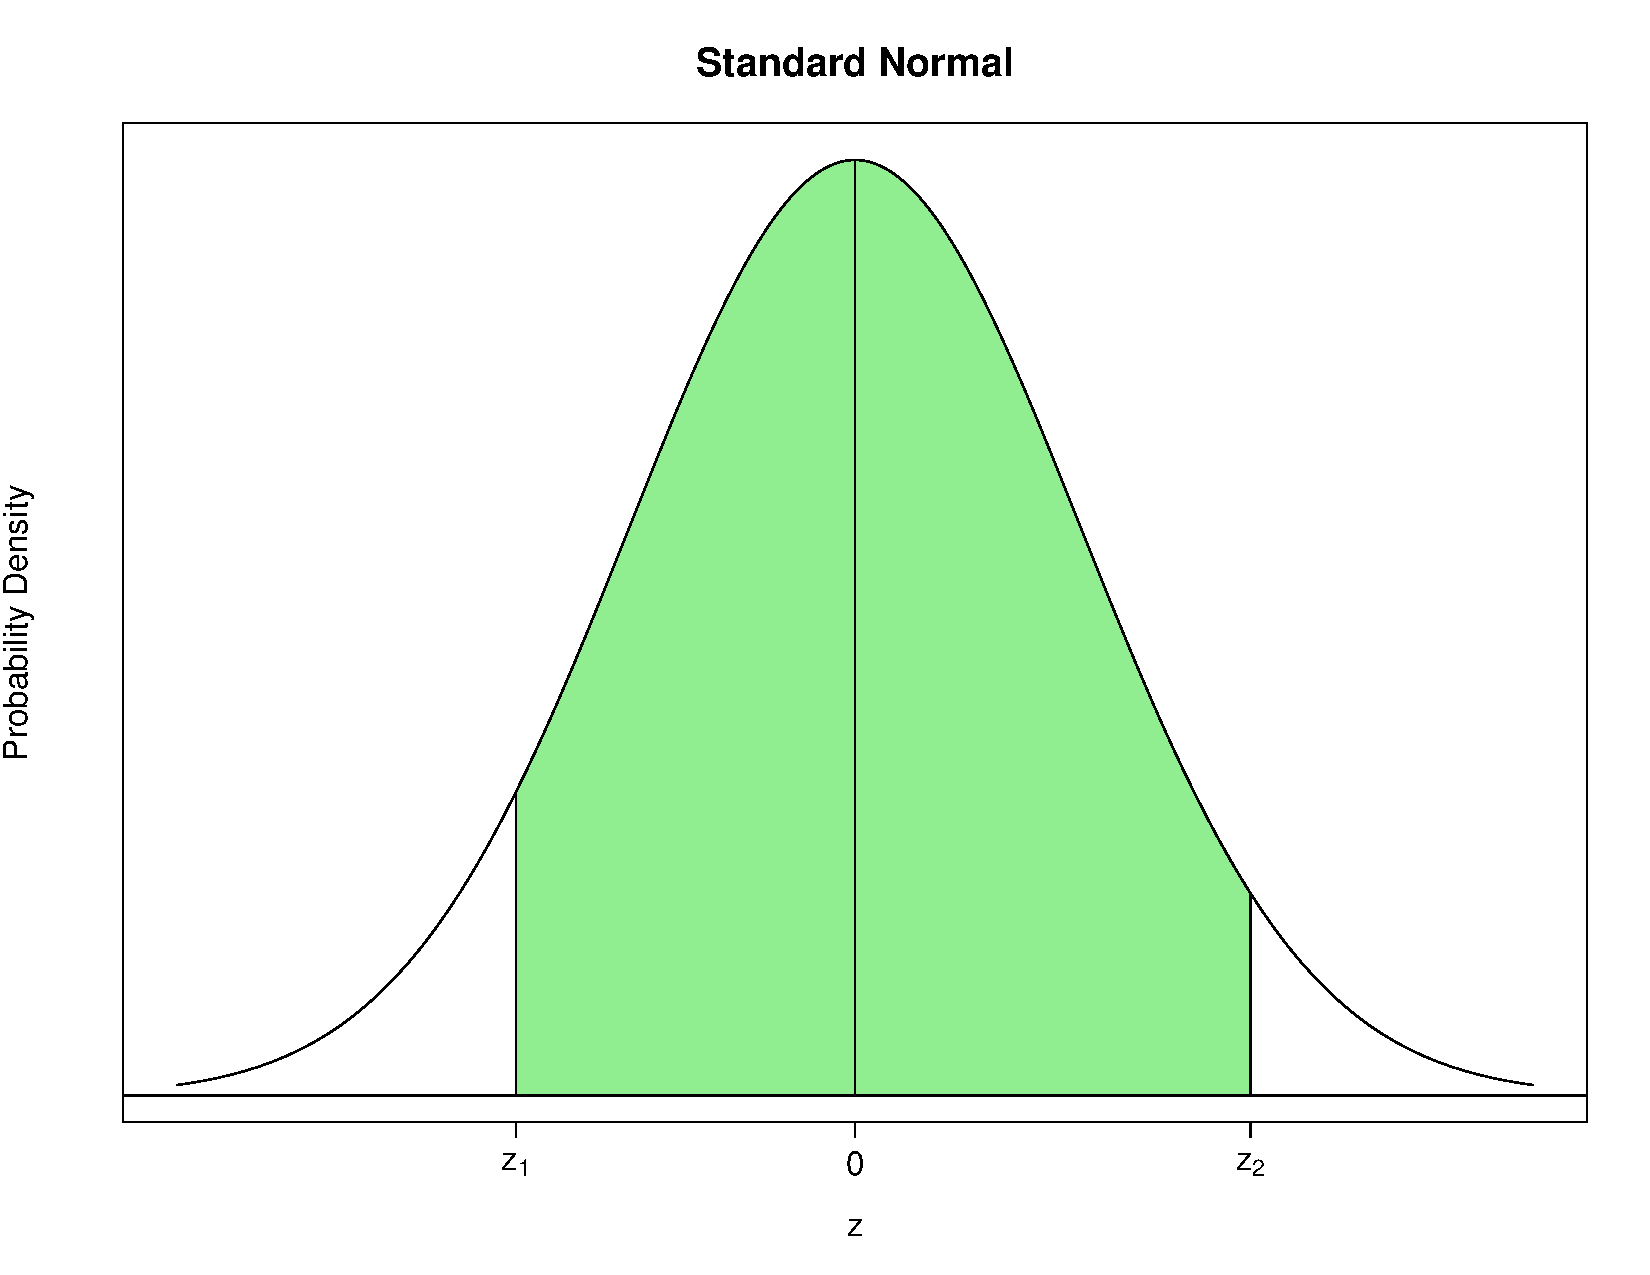
\includegraphics[width=7.250cm]{Section4/transform_st_normal.pdf}
\put (-540, 75.0){\makebox[0.7\textwidth][r]{ $\xrightarrow{\text{~Transform~}}$ }}
\end{center}

%\vspace*{-0.35cm}
~\quad We want to know:	\hspace{6.15cm}	We find:\\
\begin{center}
\begin{tabular}{ccc}
$P(x_{1} \leq X \leq x_{2})$	
	& \hspace{0.90cm}		$\xrightarrow{\text{~Convert to~}}$	\hspace{1.6cm}
	& $P(z_{1} \leq Z \leq z_{2})$\\[0.25em]
(Problem: No reference table)	&	& (Reference table available)
\end{tabular}
\end{center}
\caption{	Transforming a problem for random variable $X \sim N(\mu, \sigma^{2})$ 
		into an equivalent problem in terms of $Z \sim N(0, 1)$.}
\end{figure}

\noindent
In order to transform a normal random variable, $X \sim N(\mu,\sigma^2)$ 
into a standard normal variable, $Z \sim N(0,1)$, 
we compute the $Z$ score for an observation $x$ using transformations $\ref{transformationNormalSingle}$ and $\ref{transformationNormalAverage}$.

\begin{transformation}[Normal Transformation for Single Observations]
\label{transformationNormalSingle}
Let $X \sim N(\mu, \sigma^{2})$.
The $Z$ score for a single observation $x$ is
	\begin{equation}
	z = \frac{x - \mu}{\sigma}
	\end{equation}
\end{transformation}

\begin{transformation}[Normal Transformation for Averages]
\label{transformationNormalAverage}
The $Z$ score for an average is
Let $X \sim N(\mu, \sigma^{2})$.
	\begin{equation}
	z = \frac{ \bar{x} - \mu}{\sigma/\sqrt{n}}
	\end{equation}
\end{transformation}



In Transformation $\ref{transformationNormalAverage}$ 
the denominator ($\sigma/\sqrt{n}$) is referred to as the standard error of the mean. This transformation will be used to describe sampling distributions which will be discussed in the following chapter.\\

The \textit{Empirical Rule}, also referred to as the ``68-95-99/7`` rule or the three-sigma rule, is a quick rule of thumb for 
determining the probability of falling within 1, 2, and 3 standard deviations of the mean of the normal distribution. This rule also works for well for any distribution that is approximately bell shaped. It is useful in settings where would like to make quick estimates and do not have access to a calculator or normal tables.

\begin{rules}[Empirical rule]	\index{Empirical rule}
Let $X$ be a random variable with a probability distribution that is approximately bell-shaped. Then\\

\indent
\quad	Approximately 68\% of values lie within 1 standard deviation of the mean\\[0.25em]
\indent
\quad	Approximately 95\% of values lie within 2 standard deviations of the mean\\[0.25em]
\indent
\quad	Approximately 99.7\% of values lie within 3 standard deviations of the mean\\

Formally,
\begin{eqnarray}
P (\mu - \sigma \leq x \leq \mu + \sigma)		& \approx & 0.68	\\
P (\mu - 2 \sigma \leq x \leq \mu + 2 \sigma)	& \approx & 0.95	\\
P (\mu - 3 \sigma \leq x \leq \mu + 3 \sigma)	& \approx & 0.997
\end{eqnarray}
\end{rules}



\begin{example}
If $X \sim N(5,4)$,
\begin{benumerate}
\item Find the Z-score of X.

\begin{align*}
z = \frac{x-\mu}{\sigma} = \frac{x - 5}{2}
\end{align*}

\item Find $P(X=5)$.\\
Since $X$ is a continuous random variable, the probability of a single point is zero.
\[\Rightarrow P(X=5)=0 \]

\item Find $P(X \leq 5)$ and $P(X \geq 5)$.\\
Since the mean of $X$ is $\mu = 5$ and the normal distribution is symmetric,
\[ P(X \leq 5) = P(X \geq 5) = 0.5 \]

\begin{center}
\begin{tabular}{cc}
\frame{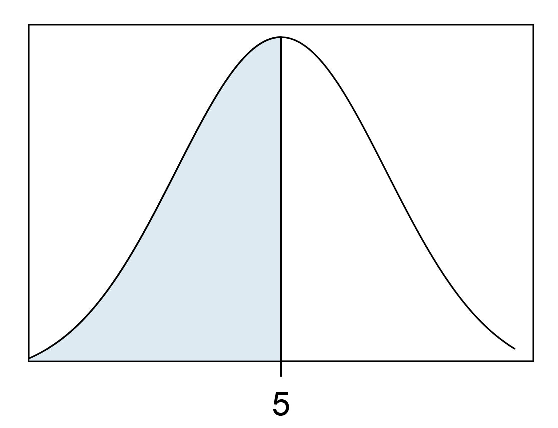
\includegraphics[scale=0.5]{Section4/xl5.pdf}}&
\frame{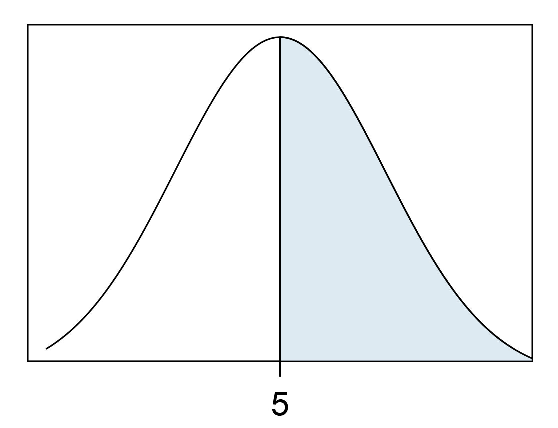
\includegraphics[scale=0.5]{Section4/xg5.pdf}}\\
$P(X \leq 5)$ & $P(X \geq 5)$
\end{tabular}
\end{center}

\item Find $P(X \leq 3)$.\\

First transform $X$ into the $Z$ statistic. When $X=3$,
\[ z = \frac{x-5}{2} = \frac{3-5}{2} = -1 \]
Therefore,
\[ P (X \leq 3) = P( Z \leq -1)\]
Using our standard normal table,
\begin{align*}
 P(Z \leq -1) = 0.159
 \Rightarrow P(X \leq 3) = 0.159
\end{align*}

\item Find $P(X \leq 7)$.

When $X=7$,
\[ z = \frac{x-5}{2} = \frac{7-5}{2} = 1 \]
Therefore,
\[ P(X \leq 7) = P(Z \leq 1) \]
Using our standard normal table,
\begin{align*}
P(Z \leq 1) = 0.841
\Rightarrow P(X \leq 7) = 0.841
\end{align*}

\item Find $P(3 \leq X \leq 7)$.\\
We want to find the probability that X is greater than 3 but less than 7. From parts (b) and (c) we know
\[P(X \leq 3) = 0.159, ~ ~ P(X \leq 7) = 0.841 \]
$P(X \leq 3)$ gives us the probability of $X$ being any number between $-\infty$ and 3. $P(X \leq 7)$ gives us the probability of $X$ being any number between $-\infty$ and 7. If we subtract $P(X \leq 3)$ from $P(X \leq 7)$, we will be left with the probability of $X$ being between 3 and 7. Graphically,
\begin{center}
\begin{tabular}{ccc}
\frame{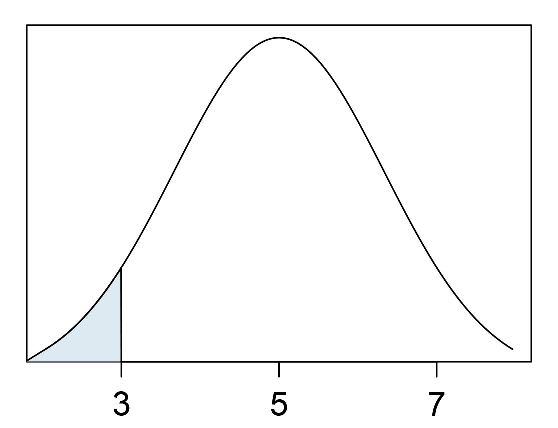
\includegraphics[scale=0.5]{Section4/3xplot.pdf}}&
\frame{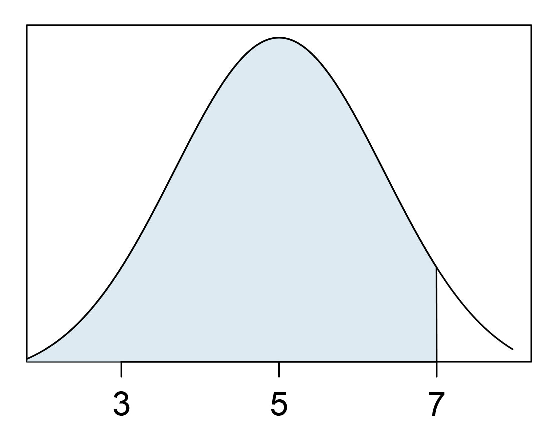
\includegraphics[scale=0.5]{Section4/x7plot.pdf}}&
\frame{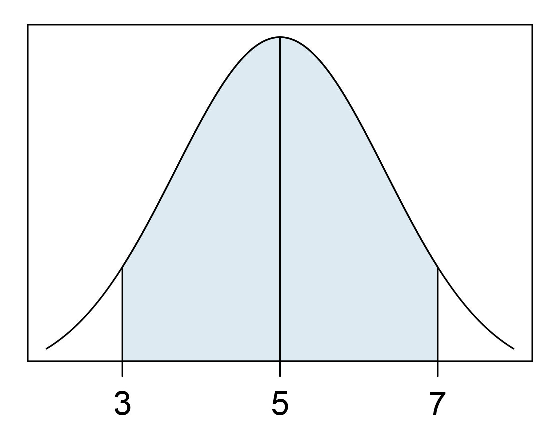
\includegraphics[scale=0.5]{Section4/3x7plot.pdf}}\\
$P(X \leq 3)$ & $P(X \leq 7)$ & $P(3 \leq X \leq 7)$
\end{tabular}
\end{center}

\begin{align*}
\Rightarrow P(3 \leq X \leq 7) &= P(X \leq 7) - P(X \leq 3) \\
				&= 0.841 - 0.159 = 0.682 
\end{align*}
Alternatively, we could recognize that $\mu - \sigma = 5 - 2 = 3$ and $\mu + \sigma = 5+2 = 7$. By the \textit{three-sigma rule} we know that $P(\mu - \sigma \leq x \leq \mu + \sigma) \approx 0.68$.

\item If $n=25$, find the Z-score of $\bar{X}$.
\[ z = \frac{\bar{x} - \mu}{\sigma/\sqrt{n}} = \frac{\bar{x} - 5}{2/\sqrt{25}} = \frac{\bar{x}-5}{2/5} = \frac{\bar{x} - 5}{0.40}\]

\item Find $P(\bar{X} \leq 4 \cup \bar{X} \geq 6)$.\\
Recall the \textit{additive property},
\[ P(A \cup B) = P(A) + P(B) - P(A \cap B)\]
Since it is impossible for $\bar{X}$ to be less than 4 and greater than 6 at the same time,
\[ P(\bar{X} \leq 4 \cap \bar{X} \geq 6) = 0 \]
Therefore,
\[ P(\bar{X} \leq 4 \cup \bar{X} \geq 6) = P(\bar{X} \leq 4) + P(\bar{X} \geq 6)\]

Plugging in $\bar{X}=4$ and $\bar{X} =6$ into our Z-score equation from part (g) yields
\begin{align*}
z = \frac{\bar{x}-5}{0.40} = \frac{4-5}{0.40} = -2.5\\
\Rightarrow P(\bar{X} \leq 4) = P(Z \leq -2.5)
\end{align*}
and
\begin{align*}
z = \frac{\bar{x}-5}{0.40} = \frac{6-5}{0.40}=2.5\\
\Rightarrow P(\bar{X} \geq 6) = P(Z \geq 2.5)
\end{align*}
Due to the symmetry of the normal distribution,
\[P(Z \geq 2.5) = P(Z \leq -2.5)\]

\begin{center}
\begin{tabular}{cc}
\frame{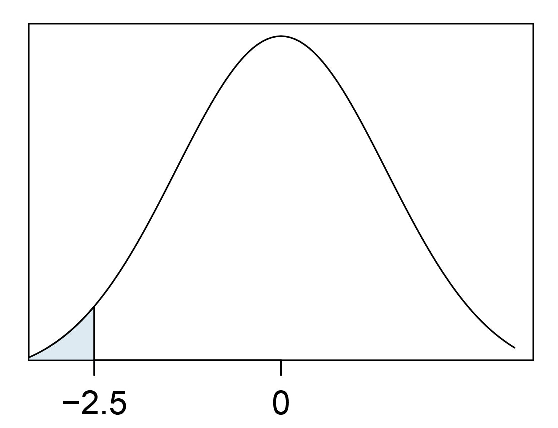
\includegraphics[scale=0.5]{Section4/zleq25.pdf}}&
\frame{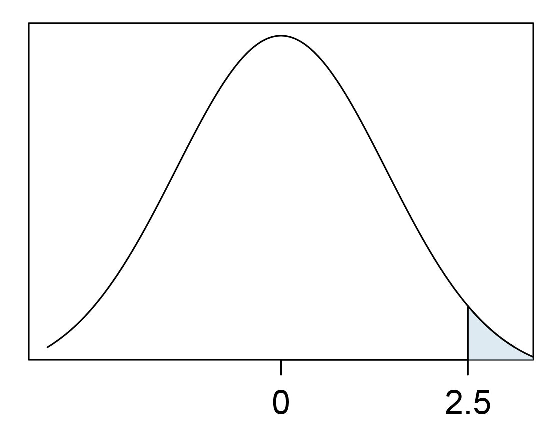
\includegraphics[scale=0.5]{Section4/zgeq25.pdf}}\\
$P(Z \leq -2.5)$ & $P(Z \geq 2.5)$
\end{tabular}
\end{center}

Using our standard normal table,
\begin{align*}
P(\bar{X} \leq 4 \cup \bar{X} \geq 6) 
&= P(\bar{X} \leq 4) + P(\bar{X} \geq 6) \\
&= P(Z \leq -2.5) + P(Z \leq -2.5) \\
&= 0.00621 + 0.00621 \\
&= 0.01242
\end{align*}



\end{benumerate}
\end{example}

\begin{example}
The corn ethanol industry is worried that unfavourable weather will lead to low crop yields in the next year. Researchers determine that yearly North American corn yield under similar weather conditions is normally distributed with a mean of 17.5 billion bushels and a standard deviation of 10 billion bushels. 

\begin{benumerate}
\item The industry puts out a statement saying that crop yield needs to remain at or above 15 billion bushels to support current demand. What is the probability that crop yield drops below 15 billion bushels?

First we find our Z statistic.
\[ z = \frac{x - \mu}{\sigma} = \frac{15 - 17.5}{10} = -0.25\]
Using our standard normal table,
\[ P(X < 15) = P(Z < -0.25) = 0.4013 \]

The probability that crop yield drops below 15 billion bushels is 0.4013.

\item If corn yields do fall below levels needed to support current demand, the industry would like to know by how much. What is the probability that corn yields are greater than 10 billion bushels given they are less than 15 billion bushels?

We are interested in finding $P(X>10|X<15)$. Via Bayes' Theorem,
\[ P(X>10|X<15) = \frac{P(X>10 \cap X<15)}{P(X<15)} = \frac{P(10<X<15)}{P(X<15)} \]

From part (a) we know that $P(X<15) = 0.4013$. Then
\begin{align*}
P(10 < X < 15) &= P(X<15) - P(X<10) = 0.4013 - P\left(Z< \frac{10-17.5}{10}\right)\\ & = 0.4013 - P(Z<-0.75) = 0.4013 - 0.2266 =0.1747
\end{align*}
Plugging this into Bayes' Theorem,

\[ P(X>10|X<15) = \frac{P(10<X<15)}{P(X<15)} =\frac{0.1747}{0.4013} = 0.4353\]
\item If 3 years are randomly sampled, what is the probability mean corn yield of these 3 years is between 10 billion and 20 billion bushels?

We need to find $P(10 \leq \bar{X} \leq 20)$.
\begin{equation}
P(10 \leq \bar{X} \leq 20) = P(\bar{X} \leq 20) - P(\bar{X} \leq 10) \\
\end{equation}
For $\bar{x}=20$,
\[ z = \frac{\bar{x}-\mu}{\sigma/ \sqrt{n}} = \frac{20 - 17.5}{10/\sqrt{3}} \approx 0.43 \]
Using our standard normal table,
\[ P(Z < 0.43) = 0.6664 \]
For $\bar{x} = 10$, 
\[ z = \frac{\bar{x}-\mu}{\sigma/ \sqrt{n}} = \frac{10 - 17.5}{10/\sqrt{3}} \approx -1.30 \]
Using our standard normal table,
\[ P(Z < -1.30) = 0.0968 \]
Putting it all together,
\[
P(10 \leq \bar{X} \leq 20) = P(Z < 0.433) - P(Z<-1.30) = 0.6664-0.0968 = 0.5698
\]
\end{benumerate}
\end{example}


\subsection{$t-$Distribution}
\label{sectiontDistribution}
\index{Distribution!t-distribution}

The Student's $t-$distribution or t distribution for short, is a continuous family of 
distributions that are commonly used in statistical inference techniques, 
particularly when the population standard deviation $\sigma$ is not known. Generally, the $t-$distribution has a bell shape similar to the normal distribution, however the thickness of the tails of the $t-$distribution varies.

\begin{nt}
The $t-$distribution was developed by William Sealy Gosset while working on quality control for the Guinness Brewery in Dublin, Ireland. He was not allowed to publish his results as Guinness did not want competitors to obtain information about the research conducted at Guinness. Gosset secretly published his work under the pseudonym {\em{student}}.
\end{nt}


The $t-$distribution is centered at zero and depends on the {\em{degrees of freedom}}. The degrees of freedom, $df$, describe the bell shape form of the $t-$distribution and the thickness of its tails.

\begin{definition}[Degrees of Freedom]
\index{Degrees of freedom}
The degrees of freedom refer to the number of free values that we can vary in the calculation of an estimate.
\end{definition}

\begin{example}
Recall the sample standard deviation is calculated using
	\begin{equation}
	s = \sqrt{ \frac{ \displaystyle\sum_{i=1}^{n} (x_{i} - \bar{x})^{2} }{ n-1 } }
	\end{equation}

In order to calculate $s$ we first calculate the mean of the sample, $\bar{x}$, then calculate the sum of the squared deviations of each observations from $\bar{x}$. There are $n$ squared deviations but only $(n - 1)$ of them are free to assume any value. This is because one $(x_{i} - \bar{x})^{2}$ must include a value of $x_{i}$ such that $\frac{ \sum_{i=1}^{n} x_{i} }{n} = \bar{x}$ that was calculated. All of the other $(n - 1)$ values of $(x_{i} - \bar{x})^{2}$ can take any value (in theory). As such $s$ is said to have $n-1$ degrees of freedom. For example, if it is known that $n=3$, $\bar{x}=5$, $x_1=6$, and $x_2=5$, $x_3$ must be fixed at 4 in order for our calculation of $\bar{x}=5$ to hold. 
\end{example}

\begin{figure}[H]
\label{figuretdist}
\begin{center}
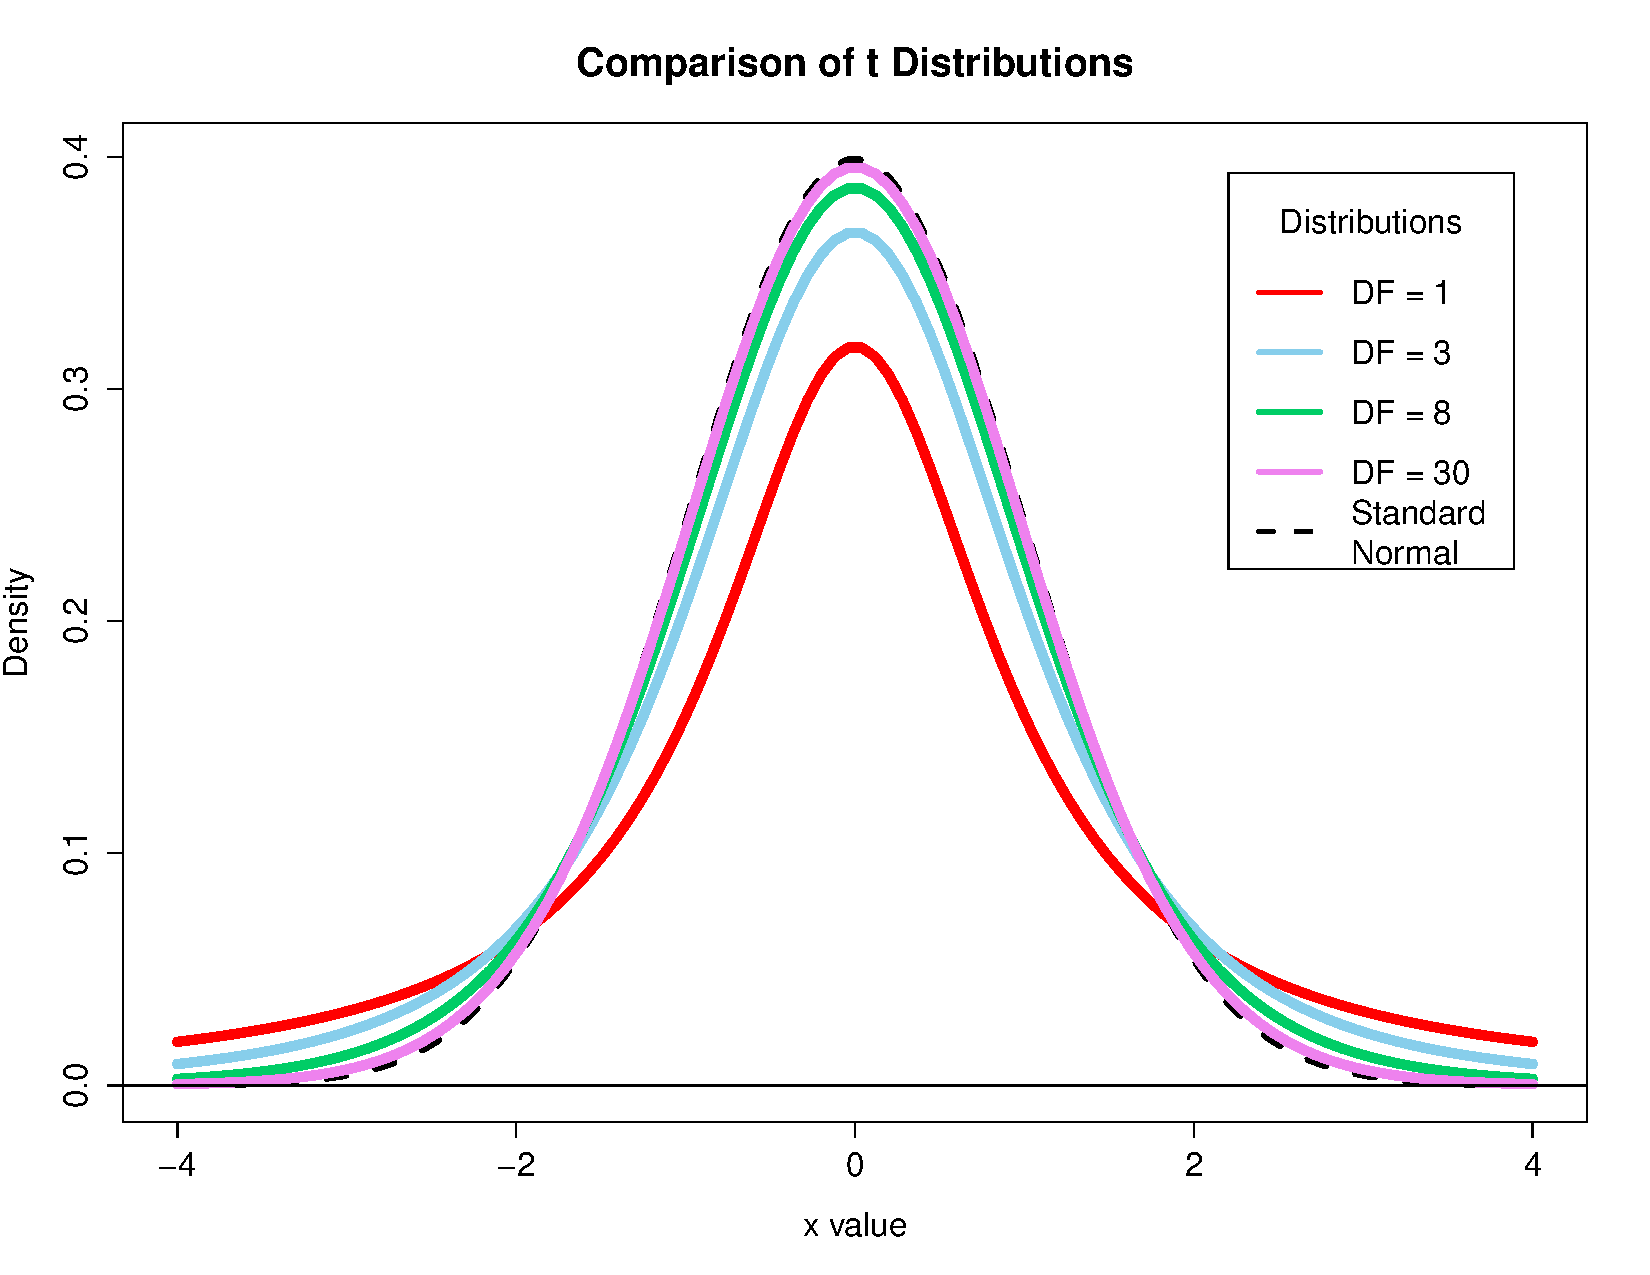
\includegraphics[scale=0.50]{Section4/tdistrs.pdf} 
\end{center}
\vspace*{-0.5cm}
\caption{Several $t-$distributions for 1,3,8 and 30 degrees of freedom along with the
standard normal distribution.}
\end{figure}

\noindent
Notice that the $t-$distribution has thicker tails than the normal distribution in general. As the degrees of freedom approach infinity, the $t$-distribution approaches the standard normal distribution.

\begin{nt}
The degrees of freedom of a distribution can be any positive real value. They do not need to by positive integers.
\end{nt}

We use the {\color{red}{$t-$table in Appendix ???} } to read values in the tails of the $t-$distribution.


\begin{example}
Assuming the sample is of size $n=10$, use the t-distribution table to determine the following.

\begin{benumerate}
\item Find $P(t \leq 0)$ and $P(t \geq 0)$.\\
The mean of the t-distribution is 0 and therefore $P(t \leq 0) = P(t \geq 0) = 0.5$.

\item Find $P(t \leq 2.262)$ and $P(t \geq 2.262)$. \\
Since $n=10$,
\[ df = n-1 = 10 -1 =9\]
To find $P(t \leq 2.262)$, we find the row that matches our degrees of freedom and move right until we find the column containing 2.262. Once we find 2.262, we move up the column until we hit the probability. Using our table yields $P(t \leq 2.262) = 0.975$. Therefore, $P(t \geq 2.262) = 1 - 0.975= 0.025$.

\item Find $P(t \leq 2)$. \\
We notice that the value of 2 is not present in the $df=9$ row. In order to estimate $P(t \leq 2)$, we determine the closest number above and below 2. In this case it would be 1.833 and 2.262. We find the $P(t \leq 1.833)$ and $P(t \leq 2.262)$ and average them to estimate $P(t \leq 2)$. 
\[ P(t \leq 2) = \frac{0.95+0.975}{2} = 0.9625 \]

\item Find $P( t \geq -0.883)$.
\[P( t \geq -0.883) = P(t \leq 0.883)\]
Using our table,
\[P( t \leq -0.883) = P( t \geq -0.883)=0.80 \]

\item Find the value $q$ such that $P(t \leq q) = 0.95$.\\
We find the column for the 95\% percentile and match it with the row representing $df=9$. This value is $q=1.833$.

\item Find the value $q$ such that $P(t \geq q) = 0.90$.\\
Due to the symmtery of the t-distribution, we know $P(t \geq q) = P(t \leq -q) = 0.90$.  We find the column for the 90\% percentile and match it with the row representing $df=9$. This value is $q=1.383$. Since $P(t \geq q) = P(t \leq -q)$, $P(t \geq -1.383) = 0.90$.

\item Find the value $q$ such that $P(t \leq q) = 0.825$.\\
We notice that there is no 82.5\% percentile column in our table. Therefore we go to the nearest percentile above and below the one of interest. That is, 80\% and 85\%. We then take the average of the two numbers corresponding to these percentiles in the $df=9$ row to approximate $q$,
\[q = \frac{0.883+1.100}{2}=0.9915\]
\end{benumerate}
\end{example}





%%\pagenumbering{arabic}\setcounter{page}{1}
%\chapter{Random variables I:  discreet}
%%start relabeling as 2.1 etc
%\pagestyle{myheadings}  \markboth{\ref{sec.matrix}.
%\titleref{sec.matrix}}{}
%\setcounter{equation}{0}
%\section{Basic Definitions}
%%\begin{frame}[<+->] \frametitle{Preliminaries}
%
%\noindent A \textbf{random variable} is the realization of what we previously called an experiment. %\pause
%
%\medskip
%
%\noindent A random variable can take on discrete values in which it will be called a \textbf{discrete}
%random variable. %\pause
%
%\medskip
%
%\noindent  A random variable can take on continuous values in which it will be called a
%\textbf{continuous} random variable.  %\pause
%
%\medskip
%
%\noindent  We often denote by $x$, or $X$ as the random variable which can be either
%discrete or continuous depending on context.
%
%%\end{frame}
%
%%\begin{frame}[<+->] \frametitle{Examples of discrete random variables}
%
%\noindent The number of sales made by a salesperson in a given week, $x=0,1,2,\ldots $. %\pause
%
%\medskip
%
%\noindent The number of consumers in a sample of 100 who favour one product over
%another, $x=0,1,\ldots, 100$. %\pause
%
%\medskip
%
%\noindent  The number of customers waiting (in minutes) to be served at a bank, $x$.
%%\end{frame}
%
%%\begin{frame}[<+->] \frametitle{Examples of continuous random variables}
%
%\noindent  The foreign exchange rate over a trading day, $x \geq 0$. %\pause
%
%\medskip
%
%\noindent  The price of Apple stocks over a trading day , $x \geq 0$. %\pause
%
%\medskip
%
%\noindent  The time it takes to log onto a popular website, $x \geq 0 $.
%%\end{frame}
%
%\section{Discrete probabilities}
%
%
%%\begin{frame}[<+->] \frametitle{Discrete Probabilities}
%
%\noindent The \textbf{discrete probability distribution}  for a discrete random variable
%$x$ consists of individual probabilities with the following properties: %\pause
%
%\begin{itemize}
%
%\item $p(x) \geq 0$ for all $x$
%
%\item $\sum p(x) = 1$
%
%\end{itemize}
%
%\noindent  Note that we are being vague in terms of the full range of $x$'s as we can have
%them to be finite or infinite. %\pause
%
%\medskip
%
%\noindent  Any probability statements will be enclosed in terms of $P$ where the individual
%probabilities will use $p$.
%
%%\end{frame}
%
%\subsection{Examples}
%
%%\begin{frame} \frametitle{Examples}%\pause
%
%Will be discussed in class.
%
%%\end{frame}
%
%%\begin{frame}[<+->] \frametitle{Population means variances and standard deviations}
%
%\noindent For a discrete random variable
%$x$ with probabilities $p(x) \geq 0$ for all $x$
%and  $\sum p(x) = 1$,
%the \textbf{mean}, or \textbf{expected value}, or \textbf{expectation} is
%$$\mu = \E(x) = \sum xp(x)$$ %\pause
%
%%\medskip
%
%\noindent The \textbf{variance} of a discrete random variable is
%$$\sigma^2 = \E \left\{(x-\mu)^2\right\} = \sum (x-\mu )^2 p(x)$$
%
%%\medskip
%
%\noindent The \textbf{standard deviation} of a discrete random variable is
%$$\sigma = \sqrt{\sum (x-\mu )^2 p(x)}$$
%
%%\end{frame}
%
%%\begin{frame}[<+->] \frametitle{A simpler formula for variance}
%
%\noindent Consider a discrete random variable
%$x$ with probabilities $p(x) \geq 0$ for all $x$ so that
%$$ \sum p(x) = 1 \mbox{ and } \mu = \sum xp(x) $$
%
%%\medskip
%
%\noindent The variance of a discrete random variable has a simpler formula: %\pause
%\begin{eqnarray*}
%\sigma^2 &=& \sum (x-\mu )^2 p(x)\\ %\pause
%&=& \sum (x^2-2\mu x + \mu^2 ) p(x)\\ %\pause
%&=& \sum x^2 p(x) -2\mu \sum x p(x)  + \mu^2  \sum p(x)\\ %\pause
%&=& \sum x^2 p(x) -2\mu^2  + \mu^2 \\ %\pause
%&=& \sum x^2 p(x) - \mu^2
%\end{eqnarray*}
%
%
%%\end{frame}
%
%\subsection{Examples}
%
%%\begin{frame} \frametitle{Examples}%\pause
%
%Will be discussed in class.
%
%%\end{frame}
%
%
%
%%\begin{frame}[<+->] \frametitle{Population parameters and empirical rules}
%
%\noindent The $\mu$, $\sigma^2$, and $\sigma$ are examples of what are called
%\textbf{population parameters}, or just \textbf{parameters}.%\pause
%
%\begin{center}
%\begin{tabular}{ccc}
%Probabilities&Chebyshev's Rule &Empirical Rule \\
%for $x$& (Emprical Rule I)& (Empirical Rule II)\\ \hline
%$P(\mu-\sigma < x < \mu +\sigma )$&$\geq 0$&0.68\\
%$P(\mu-2 \sigma < x < \mu +2 \sigma )$&0.75&0.95\\
%$P(\mu-3\sigma < x < \mu +3\sigma )$&0.89&0.99\\
%\end{tabular}
%\end{center}%\pause
%
%
%%\end{frame}
%
%\subsection{Examples}
%
%%\begin{frame} \frametitle{Examples}%\pause
%
%Will be discussed in class.
%
%%\end{frame}
%\subsection{Exercises}

\begin{enumerate}
\item  The random variable $X$ has discrete probability distribution as follows:
\begin{center}
\begin{tabular}{ccccccc}\hline
X             &2       &4        &6        &8       &10\\ \hline
$p(x)$        &0.1c    &0.2c     &0.4c     &0.2c    &0.1c\\ \hline
\end{tabular}
\end{center}
\begin{enumerate}
\item Find the value of c.
\item Find $P(X=6)$.
\item Find $P(X \geq 3)$.
\item Find $P(X > 4)$.
\item Find $P(X \leq 8)$.
\end{enumerate}
\item  A discrete random variable $X$ can assume five possible values and its distribution is shown here:
\begin{center}
\begin{tabular}{ccccccc}\hline
X             &2       &3        &5        &8       &10\\ \hline
$p(x)$        &0.15    &0.10     &-        &0.25    &0.25\\ \hline
\end{tabular}
\end{center}


\begin{enumerate}
\item Find $P(X=5)$.
\item What is the probability that x is great that 4 and 8?
\item Find $P(X \geq 3)$.
\item Find $P(X < 4)$.
\end{enumerate}

\item  Toss four fair coins and let $X$ equal the number of heads observed.

\begin{enumerate}
\item Calculate $p(x)$ for all possible values of $X$.
\item Find $P$($X=2$ or $X=3$).
\item Find $P(X \geq 3)$.
\item Find $P(X < 2)$.
\end{enumerate}

\item Consider the probability distribution shown here:

\begin{center}
\begin{tabular}{ccccccc}\hline
X             &0       &1      &2 \\ \hline
$p(x)$        &0.3    &0.4     &0.3 \\ \hline
\end{tabular}
\end{center}

\begin{center}
\begin{tabular}{ccccccc}\hline
X             &0       &1      &2 \\ \hline
$p(x)$        &0.05    &0.9     &0.05 \\ \hline
\end{tabular}
\end{center}

\begin{enumerate}
\item Calculate $\mu$ and $\sigma$ for each distribution.
\item Which distribution appears to be more variable?
\end{enumerate}

\end{enumerate}



\iffalse
a) $3x-5y=4$\\
b) $4x-7y=9$\\
c) $2x_1-3x_2+5x_3=8$

\item Determine if\\ a)$x_1=0,x_2=1,x_3=-1$\\  b)$x_1=-1,x_2=-1,x_3=6$\\ is a solution to the following
systems\\
(i)
$$\begin{array}{rrr}
x_1+3x_2+2x_3&=&1\\
x_1+x_2+3x_3&=&1\\
2x_1+4x_2+3x_3&=&-1
\end{array}$$

(ii)
$$\begin{array}{rrr}
x_1+3x_2+x_3&=&2\\
3x_1+2x_2+x_3&=&1
\end{array}$$

(iii)
$$\begin{array}{rrr}
4x_1+-3x_2+x_3&=&5\\
-5x_1+9x_2+2x_3&=&8\\
2x_1-7x_2-x_3&=&-1
\end{array}$$

\item Write the systems in question 2) as augmented matrices.

\item Put the following augmented matrices  in\\
i) row echelon form\\
ii) reduced row echelon form\\
a)$\left [\begin {array}{rrrr} 2&5&\vline&3\\1&3&\vline&2\end {array}
\right ]$
b)$\left [\begin {array}{rrrrrr} 1&-1&-2&1&\vline&7\\-2&1&6&-1
&\vline&-4\\2&0&-8&1&\vline&9\end {array}\right ]$

\item Solve
\begin{eqnarray*} x_1+3x_2-x_3&=&0\\
2x_1-5x_2+x_3&=&0\\ 3x_1+7x_2-2x_3&=&0 \end{eqnarray*}

\item Solve
$$\begin{array}{rrr} x_1-2x_2+2x_3+x_4&=&-5\\
x_2-2x_3-x_4&=&1\\ x_1-x_2+x_3&=&-5\\ 2x_1-2x_2+2x_3+x_4&=&-7
\end{array}$$

\item Solve
$$\begin{array}{rrr} x_1+2x_2+2x_3+7x_4&=&1\\
2x_1+4x_2+2x_3+9x_4&=&1\\ x_1+2x_2-x_3-x_4&=&-2\\ 3x_1+6x_2+5x_3+9x_4&=&7
\end{array}$$

\item Solve
$$\begin{array}{rrr} x_1+x_2+2x_3+3x_4+3x_5&=&2\\
x_2+2x_3+x_4&=&3\\ x_1+2x_2+4x_3+5x_4+3x_5&=&7\\ x_1-x_2-2x_3-x_4+4x_5&=&-8
\end{array}$$

\item Solve
$$\begin{array}{rrr} x_1+2x_2+x_3+x_5-x_6&=&1\\
3x_1+6x_2+6x_4+6x_6&=&12\\ x_1+2x_2+x_3-2x_5+x_6&=&2\\ 2x_1+4x_2+2x_3+2x_5-3x_6&=&-1
\end{array}$$
\end{enumerate}
\fi
\iffalse
\documentclass[12pt]{article}
\usepackage{amsmath}
\usepackage{latexsym}
\usepackage{maple2e}
\addtolength{\textwidth}{1in} \addtolength{\oddsidemargin}{-0.5in}
\addtolength{\textheight}{1.6in} \addtolength{\topmargin}{-0.8in}

\newfont{\tebbb}{msbm10 scaled\magstep1}

\newtheorem{theorem}{Theorem}[section]
\newtheorem{proposition}[theorem]{Proposition}
\newtheorem{lemma}[theorem]{Lemma}
\newtheorem{corollary}[theorem]{Corollary}
\newtheorem{remark}[theorem]{Remark}
\newtheorem{example}[theorem]{Example}
\newcommand{\beq}{\begin{equation}}
\newcommand{\eeq}{\end{equation}}
\newtheorem{definition}[theorem]{Definition}


\newcommand{\cross}[2]{{{\bf{#1}} \times {\bf{#2}}}}
\newcommand{\dotprod}[2]{{{\bf{#1}} \cdot {\bf{#2}}}}
\newcommand{\real}[1]{{\mbox{\tebbb R}}^{#1}}
\newcommand{\norm}[1]{\|{\bf{#1}}\|}
\renewcommand{\theequation}{\thesection.\arabic{equation}}

\baselineskip = 20pt plus 3pt minus 3pt

%\begin{document}
\fi
\iffalse
\section{Suggested Exercises}
\label{ssec.sugexercises}
\markright{\ref{ssec.sugexercises}
\titleref{ssec.sugexercises}}
\begin{enumerate}
\item  Find the general solution to:\\
a) $3x-5y=4$\\
b) $4x-7y=9$\\
c) $2x_1-3x_2+5x_3=8$

\item Determine if\\ a)$x_1=0,x_2=1,x_3=-1$\\  b)$x_1=-1,x_2=-1,x_3=6$\\ is a solution to the following
systems\\
(i)
$$\begin{array}{rrr}
x_1+3x_2+2x_3&=&1\\
x_1+x_2+3x_3&=&1\\
2x_1+4x_2+3x_3&=&-1
\end{array}$$

(ii)
$$\begin{array}{rrr}
x_1+3x_2+x_3&=&2\\
3x_1+2x_2+x_3&=&1
\end{array}$$

(iii)
$$\begin{array}{rrr}
4x_1+-3x_2+x_3&=&5\\
-5x_1+9x_2+2x_3&=&8\\
2x_1-7x_2-x_3&=&-1
\end{array}$$

\item Write the systems in question 2) as augmented matrices.

\item Put the following augmented matrices  in\\
i) row echelon form\\
ii) reduced row echelon form\\
a)$\left [\begin {array}{rrrr} 2&5&\vline&3\\1&3&\vline&2\end {array}
\right ]$
b)$\left [\begin {array}{rrrrrr} 1&-1&-2&1&\vline&7\\-2&1&6&-1
&\vline&-4\\2&0&-8&1&\vline&9\end {array}\right ]$

\item Solve
\begin{eqnarray*} x_1+3x_2-x_3&=&0\\
2x_1-5x_2+x_3&=&0\\ 3x_1+7x_2-2x_3&=&0 \end{eqnarray*}

\item Solve
$$\begin{array}{rrr} x_1-2x_2+2x_3+x_4&=&-5\\
x_2-2x_3-x_4&=&1\\ x_1-x_2+x_3&=&-5\\ 2x_1-2x_2+2x_3+x_4&=&-7
\end{array}$$

\item Solve
$$\begin{array}{rrr} x_1+2x_2+2x_3+7x_4&=&1\\
2x_1+4x_2+2x_3+9x_4&=&1\\ x_1+2x_2-x_3-x_4&=&-2\\ 3x_1+6x_2+5x_3+9x_4&=&7
\end{array}$$

\item Solve
$$\begin{array}{rrr} x_1+x_2+2x_3+3x_4+3x_5&=&2\\
x_2+2x_3+x_4&=&3\\ x_1+2x_2+4x_3+5x_4+3x_5&=&7\\ x_1-x_2-2x_3-x_4+4x_5&=&-8
\end{array}$$

\item Solve
$$\begin{array}{rrr} x_1+2x_2+x_3+x_5-x_6&=&1\\
3x_1+6x_2+6x_4+6x_6&=&12\\ x_1+2x_2+x_3-2x_5+x_6&=&2\\ 2x_1+4x_2+2x_3+2x_5-3x_6&=&-1
\end{array}$$
\end{enumerate}



\section{Answers to activity questions and suggested
exercises}\label{ssec.answers1}\markright{\ref{ssec.answers1}
\titleref{ssec.answers1}}

{\bf Activity Questions}

\bigskip

\noindent {\bf \ref{ssec.lineq}:}
\begin{enumerate} \item \begin{enumerate}
\item[(i)] linear
\item[(ii)] non-linear
\item[(iii)] non-linear
\end{enumerate}
\item \begin{enumerate}
\item[(i)] $\{(s, \ t, \ 2-4s+t): \ s,t  \ \in \mbox{\tebbb R}\}$,
There are an infinite number of particular solutions, an example
is $x=1,\ y=0,\ z=3$, which is found by letting $t=1$ and $s=0$.
\item[(ii)] $\{(s, \ t, \ u, \ 2-s+t-6u): \ s,t,u  \ \in \mbox{\tebbb
R}\}$. An example of a particular solution is
$x_1=1, \ x_2=1, \ x_3=0,\ x_4=2$ which is found by letting
$s=1,\ t=1,\ u=0$.
\end{enumerate}
\end{enumerate}

\noindent {\bf \ref{ssec.mlinsys}}
\begin{enumerate}
\item $\left [ \begin{array}{rrrrcr}
                    1&-2&1&2&\vline&5 \\
                    -1&0&-1&0&\vline&-5 \\
                    0&1&-1&-2&\vline&-1 \end{array} \right ]$

\item $\left[ \begin{array}{rrrr}
1&-2&1&2 \\ -1&0&-1&0 \\ 0&1&-1&-2 \end{array} \right]
\left[\begin{array}{r} x_1 \\ x_2 \\ x_3 \\ x_4
\end{array} \right]=\left[ \begin{array}{r} 5 \\ -5 \\ -1
\end{array} \right]$

\end{enumerate}
$\left[ \begin{array}{rrrr} 1&-2&1&2 \\ -1&0&-1&0 \\ 0&1&-1&-2
\end{array} \right]$ is the coefficient matrix.

\bigskip

\noindent {\bf \ref{ssec.rreduction}}
\begin{enumerate}
\item divide row 2 by 2
$$\left \{ \begin{array}{rrrrrrr}
x&+&y&+&3z&=&-2\\
&&2y&-&z&=&4
\end{array} \right . \quad \leadsto \quad \left \{
\begin{array}{rrrrrrr}
x&+&y&+&3z&=&-2\\ &&y&-&\frac{1}{2}z&=&2
\end{array} \right .$$

\item interchange row 2 and 3
$$\left \{ \begin{array}{rrrrrrr}
x&+&0.1y&+&3z&=&-2\\
2x&&&-&z&=&4\\
6x&-&y&-&2z&=&1 \end{array} \right .  \leadsto
\left \{ \begin{array}{rrrrrrr}
x&+&0.1y&+&3z&=&-2\\
6x&-&y&-&2z&=&1 \\
2x&&&-&z&=&4
\end{array} \right .$$

\item row 2 minus 2 times row 1
$$\left \{ \begin{array}{rrrrr}
x&-&y&=&2\\
2x&+&y&=&1 \end{array} \right . \quad \leadsto \quad
\left \{ \begin{array}{rrrrr}
x&-&y&=&2\\
&&3y&=&-3 \end{array} \right .$$
\end{enumerate}

\bigskip

\noindent {\bf \ref{ssec.gausse}:}

\noindent {\bf (a)} \begin{enumerate}
\item $ \left [ \begin{array}{rrrcr}
                    1&-1&0&\vline&\frac{3}{2}\\
                    0&1&0&\vline&\frac{1}{2}\\
                    0&0&1&\vline&-1 \end{array} \right ]$
\item $\left [ \begin{array}{rrrrcr} 1 &-1 &-2&3&\vline&-1\\
0&0&1&
-1&\vline&2
\end{array} \right ].$
\end{enumerate}
{\bf (b)} \begin{enumerate}
\item $ \left [ \begin{array}{rrrcr}
                    1&0&0&\vline&2\\
                    0&1&0&\vline&\frac{1}{2}\\
                    0&0&1&\vline&-1 \end{array} \right ].$
\item $\left [ \begin{array}{rrrrcr} 1&-1&0&1&\vline&3\\0&0&1&-1&\vline&2
\end{array} \right ]$.
\end{enumerate}
{\bf (c)} \begin{enumerate}
\item $x_1=2,\ x_2=\frac{1}{2}, \ x_3=-1$.
\item $x_1=3+s-t, \ x_2=s, \ x_3=2+t, \ x_4=t$.
\end{enumerate}

\bigskip

\noindent {\bf Suggested Exercises}

\begin{enumerate}
\item
a) $\{(\frac{4}{3}+\frac{5}{3}t,t): t \in {\mbox{\tebbb R}}\}$\\
b) $\{(t,-\frac{9}{7}+\frac{4}{7}t): t \in {\mbox{\tebbb R}}\}$\\
c)  $\{(s, t,\frac{8}{5}-\frac{2}{5}s+\frac{3}{5}t): s,t \in {\mbox{\tebbb R}}\}$
\item
a) (i)no, (ii) yes, (iii) no,\\
b) (i)no, (ii) yes, (iii) yes,\\

\item a) $\left [\begin {array}{rrrrr} 1&3&2&\vline&1 \\ 1&1&3&\vline&1\\ 2&4&3&
\vline&-1  \end {array}\right ]$, b)$\left [\begin {array}{rrrrr} 1&3&1&\vline&2 \\3&2&1&
\vline&1\end {array}\right ]$, c)$\left [\begin {array}{rrrrr} 4&-3&1&\vline&5 \\-5&9&2&
\vline&8 \\ 2&-7&-1&\vline&-1\end {array}\right ]$
\item a) (i)$\left [\begin {array}{rrrr} 1&\frac{5}{2}&\vline&\frac{3}{2}\\0&1&\vline&1
\end {array}\right ]$, \quad (ii) $\left [\begin {array}{rrrr} 1&0&\vline&-1\\0&1&\vline&1\end {array}
\right ]$\\

b) (i)$\left [\begin {array}{rrrrrr} 1&-1&-2&1&\vline&7\\0&1&-2&-1&
\vline&-10\\0&0&0&1&\vline&15\end {array}\right ]$, \quad
(ii)$\left [\begin {array}{rrrrrr} 1&0&-4&0&\vline&-3\\0&1&-2&0&\vline&5
\\0&0&0&1&\vline&15\end {array}\right ]$

\item $x_1=0, x_2=0, x_3=0$
\item $x_1=-2,x_2=2,x_3=-1,x_4=3$
\item  no solution
\item $x_1=-5,x_2=1-2t,x_3=t,x_4=2,x_5=0$
\item
$x_1=-2-2s-2t,x_2=s,x_3=\frac{13}{3}+2t,x_4=t,x_5=\frac{5}{3},
x_6=3$

\end{enumerate}
\fi

%\end{document}

%
%\section{Binomial probabilities}
%
%\subsection{Motivation}
%
%%\begin{frame}
%%\frametitle{Binomial Experiments}%\pause
%
%\noindent A \textbf{binomial experiment} consists of the following:
%
%\begin{itemize}
%
%\item We have $n$ identical random variables each called a trial.
%
%\item  There are two possible outcomes for each trial, ``success" or ``failure", you can also
%think in terms of a coin toss with success being heads and failure being tails.
%
%\item  The probability of success will be $0 \leq p \leq 1$ and the probability of failure will
%be $q=1-p$.
%
%\item  Each random variable will be independent.
%
%\item  The binomial random variable $x$ is the number of success in $n$ trials.
%
%\end{itemize}
%
%%\end{frame}
%
%
%\subsection{Bionomial Distribution}
%%\begin{frame} \frametitle{Binomial Distribution}%\pause
%
%The \textbf{binomial distribution} for the discrete random variable $x=0,1,\ldots  , n$ is
%$$p(x)=
%\left(
%\begin{array}{c}
%n \\
%x
%\end{array}
%\right)
%p^x q^{n-x}
%$$
%where %\pause
%\begin{eqnarray*}
%p&=&\mbox{is the probability of success for a single trial}\\  %\pause
%q&=&1-p\\  %\pause
%n&=&\mbox{is the number of trials}\\  %\pause
%x&=&\mbox{is the number of success in n trials}\\  %\pause
%n-x&=&\mbox{is the number of failures in n trials}\\  %\pause
%\left(
%\begin{array}{c}
%n \\
%x
%\end{array}
%\right)&=&\frac{n!}{x!(n-x)!}
%\end{eqnarray*}
%
%%\end{frame}
%
%\subsection{Examples}
%
%%\begin{frame} \frametitle{Examples}%\pause
%
%Will be discussed in class.
%
%%\end{frame}
%
%%\begin{frame} \frametitle{Binomial Distribution}%\pause
%
%\noindent The mean $\mu=np$. %\pause
%
%\bigskip
%
%\noindent The variance $\sigma^2=npq$.%\pause
%
%\bigskip
%
%\noindent The standard deviation $\sigma=\sqrt{npq}$.
%
%%\end{frame}
%
%\subsection{Examples}
%
%%\begin{frame} \frametitle{Examples}%\pause
%
%Will be discussed in class.
%
%\subsection{Exercises}

\begin{enumerate}
\item  Consider the following probability distribution for $x=0,1,\ldots  , 5$:
$$p(x)=
\left(
\begin{array}{c}
5 \\
x
\end{array}
\right)
0.7^x 0.3^{5-x}
$$

\iffalse
\begin{center}
\begin{tabular}{ccccccc}\hline
X             &2       &4        &6        &8       &10\\ \hline
$p(x)$        &0.1c    &0.2c     &0.4c     &0.2c    &0.1c\\ \hline
\end{tabular}
\end{center}
\fi
\begin{enumerate}
\item Is $x$ a discrete or a continuous random variable?
\item what is the name of the probability distribution?
\item Graph the probability distribution.
\item Find the mean and standard deviation of $x$.
\item Show the mean and the 2-standard-deviation interval on each side of the mean on the graph you draw in part c.
\end{enumerate}

\item  If $x$ is a binomial random variable with $n=3$ and $p=0.3$.
\iffalse
\begin{center}
\begin{tabular}{ccccccc}\hline
X             &2       &3        &5        &8       &10\\ \hline
$p(x)$        &0.15    &0.10     &-        &0.25    &0.25\\ \hline
\end{tabular}
\end{center}
\fi

\begin{enumerate}
\item Calculate the value of $p(x)$,$x=0,1,2,3$.
\item Using the answer from part a,give the probability distribution for $x$ in tabular form.
\end{enumerate}

\item  Suppose $x$ is a binomial random variable,computer $p(x)$ ro each of the following cases:

\begin{enumerate}
\item $n=5,x=1,p=0.2$.
\item $n=3,x=0,p=0.7$.
\item $n=4,x=2,q=0.6$.
\end{enumerate}

\item  If $x$ is a binomial random variable,calculate $\mu$ and $\sigma$ ro for each of the following:

\begin{enumerate}
\item $n=25,p=0.2$.
\item $n=80,p=0.7$.
\item $n=1000,q=0.9$.
\end{enumerate}
\iffalse
\item Consider the probability distribution shown here:

\begin{center}
\begin{tabular}{ccccccc}\hline
X             &0       &1      &2 \\ \hline
$p(x)$        &0.3    &0.4     &0.3 \\ \hline
\end{tabular}
\end{center}

\begin{center}
\begin{tabular}{ccccccc}\hline
X             &0       &1      &2 \\ \hline
$p(x)$        &0.05    &0.9     &0.05 \\ \hline
\end{tabular}
\end{center}

\begin{enumerate}
\item Calculate $\mu$ and $\sigma$ for each distribution.
\item Which distribution appears to be more variable?
\end{enumerate}
\fi
\end{enumerate}



\iffalse
a) $3x-5y=4$\\
b) $4x-7y=9$\\
c) $2x_1-3x_2+5x_3=8$

\item Determine if\\ a)$x_1=0,x_2=1,x_3=-1$\\  b)$x_1=-1,x_2=-1,x_3=6$\\ is a solution to the following
systems\\
(i)
$$\begin{array}{rrr}
x_1+3x_2+2x_3&=&1\\
x_1+x_2+3x_3&=&1\\
2x_1+4x_2+3x_3&=&-1
\end{array}$$

(ii)
$$\begin{array}{rrr}
x_1+3x_2+x_3&=&2\\
3x_1+2x_2+x_3&=&1
\end{array}$$

(iii)
$$\begin{array}{rrr}
4x_1+-3x_2+x_3&=&5\\
-5x_1+9x_2+2x_3&=&8\\
2x_1-7x_2-x_3&=&-1
\end{array}$$

\item Write the systems in question 2) as augmented matrices.

\item Put the following augmented matrices  in\\
i) row echelon form\\
ii) reduced row echelon form\\
a)$\left [\begin {array}{rrrr} 2&5&\vline&3\\1&3&\vline&2\end {array}
\right ]$
b)$\left [\begin {array}{rrrrrr} 1&-1&-2&1&\vline&7\\-2&1&6&-1
&\vline&-4\\2&0&-8&1&\vline&9\end {array}\right ]$

\item Solve
\begin{eqnarray*} x_1+3x_2-x_3&=&0\\
2x_1-5x_2+x_3&=&0\\ 3x_1+7x_2-2x_3&=&0 \end{eqnarray*}

\item Solve
$$\begin{array}{rrr} x_1-2x_2+2x_3+x_4&=&-5\\
x_2-2x_3-x_4&=&1\\ x_1-x_2+x_3&=&-5\\ 2x_1-2x_2+2x_3+x_4&=&-7
\end{array}$$

\item Solve
$$\begin{array}{rrr} x_1+2x_2+2x_3+7x_4&=&1\\
2x_1+4x_2+2x_3+9x_4&=&1\\ x_1+2x_2-x_3-x_4&=&-2\\ 3x_1+6x_2+5x_3+9x_4&=&7
\end{array}$$

\item Solve
$$\begin{array}{rrr} x_1+x_2+2x_3+3x_4+3x_5&=&2\\
x_2+2x_3+x_4&=&3\\ x_1+2x_2+4x_3+5x_4+3x_5&=&7\\ x_1-x_2-2x_3-x_4+4x_5&=&-8
\end{array}$$

\item Solve
$$\begin{array}{rrr} x_1+2x_2+x_3+x_5-x_6&=&1\\
3x_1+6x_2+6x_4+6x_6&=&12\\ x_1+2x_2+x_3-2x_5+x_6&=&2\\ 2x_1+4x_2+2x_3+2x_5-3x_6&=&-1
\end{array}$$
\end{enumerate}
\fi
\iffalse
\documentclass[12pt]{article}
\usepackage{amsmath}
\usepackage{latexsym}
\usepackage{maple2e}
\addtolength{\textwidth}{1in} \addtolength{\oddsidemargin}{-0.5in}
\addtolength{\textheight}{1.6in} \addtolength{\topmargin}{-0.8in}

\newfont{\tebbb}{msbm10 scaled\magstep1}

\newtheorem{theorem}{Theorem}[section]
\newtheorem{proposition}[theorem]{Proposition}
\newtheorem{lemma}[theorem]{Lemma}
\newtheorem{corollary}[theorem]{Corollary}
\newtheorem{remark}[theorem]{Remark}
\newtheorem{example}[theorem]{Example}
\newcommand{\beq}{\begin{equation}}
\newcommand{\eeq}{\end{equation}}
\newtheorem{definition}[theorem]{Definition}


\newcommand{\cross}[2]{{{\bf{#1}} \times {\bf{#2}}}}
\newcommand{\dotprod}[2]{{{\bf{#1}} \cdot {\bf{#2}}}}
\newcommand{\real}[1]{{\mbox{\tebbb R}}^{#1}}
\newcommand{\norm}[1]{\|{\bf{#1}}\|}
\renewcommand{\theequation}{\thesection.\arabic{equation}}

\baselineskip = 20pt plus 3pt minus 3pt

%\begin{document}
\fi
\iffalse
\section{Suggested Exercises}
\label{ssec.sugexercises}
\markright{\ref{ssec.sugexercises}
\titleref{ssec.sugexercises}}
\begin{enumerate}
\item  Find the general solution to:\\
a) $3x-5y=4$\\
b) $4x-7y=9$\\
c) $2x_1-3x_2+5x_3=8$

\item Determine if\\ a)$x_1=0,x_2=1,x_3=-1$\\  b)$x_1=-1,x_2=-1,x_3=6$\\ is a solution to the following
systems\\
(i)
$$\begin{array}{rrr}
x_1+3x_2+2x_3&=&1\\
x_1+x_2+3x_3&=&1\\
2x_1+4x_2+3x_3&=&-1
\end{array}$$

(ii)
$$\begin{array}{rrr}
x_1+3x_2+x_3&=&2\\
3x_1+2x_2+x_3&=&1
\end{array}$$

(iii)
$$\begin{array}{rrr}
4x_1+-3x_2+x_3&=&5\\
-5x_1+9x_2+2x_3&=&8\\
2x_1-7x_2-x_3&=&-1
\end{array}$$

\item Write the systems in question 2) as augmented matrices.

\item Put the following augmented matrices  in\\
i) row echelon form\\
ii) reduced row echelon form\\
a)$\left [\begin {array}{rrrr} 2&5&\vline&3\\1&3&\vline&2\end {array}
\right ]$
b)$\left [\begin {array}{rrrrrr} 1&-1&-2&1&\vline&7\\-2&1&6&-1
&\vline&-4\\2&0&-8&1&\vline&9\end {array}\right ]$

\item Solve
\begin{eqnarray*} x_1+3x_2-x_3&=&0\\
2x_1-5x_2+x_3&=&0\\ 3x_1+7x_2-2x_3&=&0 \end{eqnarray*}

\item Solve
$$\begin{array}{rrr} x_1-2x_2+2x_3+x_4&=&-5\\
x_2-2x_3-x_4&=&1\\ x_1-x_2+x_3&=&-5\\ 2x_1-2x_2+2x_3+x_4&=&-7
\end{array}$$

\item Solve
$$\begin{array}{rrr} x_1+2x_2+2x_3+7x_4&=&1\\
2x_1+4x_2+2x_3+9x_4&=&1\\ x_1+2x_2-x_3-x_4&=&-2\\ 3x_1+6x_2+5x_3+9x_4&=&7
\end{array}$$

\item Solve
$$\begin{array}{rrr} x_1+x_2+2x_3+3x_4+3x_5&=&2\\
x_2+2x_3+x_4&=&3\\ x_1+2x_2+4x_3+5x_4+3x_5&=&7\\ x_1-x_2-2x_3-x_4+4x_5&=&-8
\end{array}$$

\item Solve
$$\begin{array}{rrr} x_1+2x_2+x_3+x_5-x_6&=&1\\
3x_1+6x_2+6x_4+6x_6&=&12\\ x_1+2x_2+x_3-2x_5+x_6&=&2\\ 2x_1+4x_2+2x_3+2x_5-3x_6&=&-1
\end{array}$$
\end{enumerate}



\section{Answers to activity questions and suggested
exercises}\label{ssec.answers1}\markright{\ref{ssec.answers1}
\titleref{ssec.answers1}}

{\bf Activity Questions}

\bigskip

\noindent {\bf \ref{ssec.lineq}:}
\begin{enumerate} \item \begin{enumerate}
\item[(i)] linear
\item[(ii)] non-linear
\item[(iii)] non-linear
\end{enumerate}
\item \begin{enumerate}
\item[(i)] $\{(s, \ t, \ 2-4s+t): \ s,t  \ \in \mbox{\tebbb R}\}$,
There are an infinite number of particular solutions, an example
is $x=1,\ y=0,\ z=3$, which is found by letting $t=1$ and $s=0$.
\item[(ii)] $\{(s, \ t, \ u, \ 2-s+t-6u): \ s,t,u  \ \in \mbox{\tebbb
R}\}$. An example of a particular solution is
$x_1=1, \ x_2=1, \ x_3=0,\ x_4=2$ which is found by letting
$s=1,\ t=1,\ u=0$.
\end{enumerate}
\end{enumerate}

\noindent {\bf \ref{ssec.mlinsys}}
\begin{enumerate}
\item $\left [ \begin{array}{rrrrcr}
                    1&-2&1&2&\vline&5 \\
                    -1&0&-1&0&\vline&-5 \\
                    0&1&-1&-2&\vline&-1 \end{array} \right ]$

\item $\left[ \begin{array}{rrrr}
1&-2&1&2 \\ -1&0&-1&0 \\ 0&1&-1&-2 \end{array} \right]
\left[\begin{array}{r} x_1 \\ x_2 \\ x_3 \\ x_4
\end{array} \right]=\left[ \begin{array}{r} 5 \\ -5 \\ -1
\end{array} \right]$

\end{enumerate}
$\left[ \begin{array}{rrrr} 1&-2&1&2 \\ -1&0&-1&0 \\ 0&1&-1&-2
\end{array} \right]$ is the coefficient matrix.

\bigskip

\noindent {\bf \ref{ssec.rreduction}}
\begin{enumerate}
\item divide row 2 by 2
$$\left \{ \begin{array}{rrrrrrr}
x&+&y&+&3z&=&-2\\
&&2y&-&z&=&4
\end{array} \right . \quad \leadsto \quad \left \{
\begin{array}{rrrrrrr}
x&+&y&+&3z&=&-2\\ &&y&-&\frac{1}{2}z&=&2
\end{array} \right .$$

\item interchange row 2 and 3
$$\left \{ \begin{array}{rrrrrrr}
x&+&0.1y&+&3z&=&-2\\
2x&&&-&z&=&4\\
6x&-&y&-&2z&=&1 \end{array} \right .  \leadsto
\left \{ \begin{array}{rrrrrrr}
x&+&0.1y&+&3z&=&-2\\
6x&-&y&-&2z&=&1 \\
2x&&&-&z&=&4
\end{array} \right .$$

\item row 2 minus 2 times row 1
$$\left \{ \begin{array}{rrrrr}
x&-&y&=&2\\
2x&+&y&=&1 \end{array} \right . \quad \leadsto \quad
\left \{ \begin{array}{rrrrr}
x&-&y&=&2\\
&&3y&=&-3 \end{array} \right .$$
\end{enumerate}

\bigskip

\noindent {\bf \ref{ssec.gausse}:}

\noindent {\bf (a)} \begin{enumerate}
\item $ \left [ \begin{array}{rrrcr}
                    1&-1&0&\vline&\frac{3}{2}\\
                    0&1&0&\vline&\frac{1}{2}\\
                    0&0&1&\vline&-1 \end{array} \right ]$
\item $\left [ \begin{array}{rrrrcr} 1 &-1 &-2&3&\vline&-1\\
0&0&1&
-1&\vline&2
\end{array} \right ].$
\end{enumerate}
{\bf (b)} \begin{enumerate}
\item $ \left [ \begin{array}{rrrcr}
                    1&0&0&\vline&2\\
                    0&1&0&\vline&\frac{1}{2}\\
                    0&0&1&\vline&-1 \end{array} \right ].$
\item $\left [ \begin{array}{rrrrcr} 1&-1&0&1&\vline&3\\0&0&1&-1&\vline&2
\end{array} \right ]$.
\end{enumerate}
{\bf (c)} \begin{enumerate}
\item $x_1=2,\ x_2=\frac{1}{2}, \ x_3=-1$.
\item $x_1=3+s-t, \ x_2=s, \ x_3=2+t, \ x_4=t$.
\end{enumerate}

\bigskip

\noindent {\bf Suggested Exercises}

\begin{enumerate}
\item
a) $\{(\frac{4}{3}+\frac{5}{3}t,t): t \in {\mbox{\tebbb R}}\}$\\
b) $\{(t,-\frac{9}{7}+\frac{4}{7}t): t \in {\mbox{\tebbb R}}\}$\\
c)  $\{(s, t,\frac{8}{5}-\frac{2}{5}s+\frac{3}{5}t): s,t \in {\mbox{\tebbb R}}\}$
\item
a) (i)no, (ii) yes, (iii) no,\\
b) (i)no, (ii) yes, (iii) yes,\\

\item a) $\left [\begin {array}{rrrrr} 1&3&2&\vline&1 \\ 1&1&3&\vline&1\\ 2&4&3&
\vline&-1  \end {array}\right ]$, b)$\left [\begin {array}{rrrrr} 1&3&1&\vline&2 \\3&2&1&
\vline&1\end {array}\right ]$, c)$\left [\begin {array}{rrrrr} 4&-3&1&\vline&5 \\-5&9&2&
\vline&8 \\ 2&-7&-1&\vline&-1\end {array}\right ]$
\item a) (i)$\left [\begin {array}{rrrr} 1&\frac{5}{2}&\vline&\frac{3}{2}\\0&1&\vline&1
\end {array}\right ]$, \quad (ii) $\left [\begin {array}{rrrr} 1&0&\vline&-1\\0&1&\vline&1\end {array}
\right ]$\\

b) (i)$\left [\begin {array}{rrrrrr} 1&-1&-2&1&\vline&7\\0&1&-2&-1&
\vline&-10\\0&0&0&1&\vline&15\end {array}\right ]$, \quad
(ii)$\left [\begin {array}{rrrrrr} 1&0&-4&0&\vline&-3\\0&1&-2&0&\vline&5
\\0&0&0&1&\vline&15\end {array}\right ]$

\item $x_1=0, x_2=0, x_3=0$
\item $x_1=-2,x_2=2,x_3=-1,x_4=3$
\item  no solution
\item $x_1=-5,x_2=1-2t,x_3=t,x_4=2,x_5=0$
\item
$x_1=-2-2s-2t,x_2=s,x_3=\frac{13}{3}+2t,x_4=t,x_5=\frac{5}{3},
x_6=3$

\end{enumerate}
\fi

%\end{document}
` 
%
%\section{Binomial Distribution and the Empirical Rules}
%
%%\begin{frame} \frametitle{Binomial table}%\pause
%
%\noindent Tables in Appendix B
%
%\medskip
%
%\noindent 11th edition, pp.  815--817
%
%\medskip
%
%\noindent 10th edition,  pp.  875--878
%
%\medskip
%
%\noindent Fixed $n$ and varying $p'$s and $k'$s, the tables give
%$$P(x \leq k)=\sum_{x=0}^k p(x)$$
%
%%\end{frame}
%
%%\end{frame}
%\section{Summary}\label{ssec.sumry2}
%\markright{\ref{ssec.sumry2} \titleref{ssec.sumry2}}
%{\bf Section Keywords: random variable;discrete;continuous;
%discrete probability distribution;mean;expected value;
%expectation;variance;standard deviation;\\population parameters;
%parameters;binomial experiment.
%}
%%\iffalse
%%\subsection{Exercises}
%%
%%\begin{frame} \frametitle{Exercises}%\pause
%%
%%\noindent 11th edition, p.196:  4.37--4.42
%%
%%\noindent 10th edition, p.215:  4.36--4.41
%%\end{frame}
%%\fi
%%
%%
%%\iffalse
%%\subsection{Exercises}
%%
%%%\begin{frame} \frametitle{Exercises}%\pause
%%
%%\noindent 11th edition, p.183:  4.12 -- 4.18.
%%
%%\bigskip
%%
%%\noindent 10th edition, p. 200:  4.12 -- 4.18.
%%
%%%\end{frame}
%%\fi 